
\documentclass[a4paper,12pt]{article}
\usepackage{graphicx}
\usepackage[table,xcdraw]{xcolor}
\usepackage{geometry}
\usepackage{float}
\usepackage[colorlinks=false, hidelinks]{hyperref}
\usepackage{fancyhdr}% For page numbering
\geometry{top=1in,bottom=1in,left=1in,right=1in}
\usepackage{listings}
\usepackage{xcolor}
\usepackage{hyperref}
\pagestyle{empty}


\begin{document}

\begin{center}
    \vspace{0.2cm}
    \textbf{\large{Course Title: Software Engineering \& ISD Lab}}\\
    \vspace{0.2cm}
    \textbf{Course Code: CSE-404}\\
    \vspace{0.2cm}
    \textbf{4\textsuperscript{th}Year 1\textsuperscript{st}Semester Examination 2023}\\
    \vspace{0.5cm}
    \textbf{Date of Submission: \today}\\

    \vspace{1.5cm}
    
\includegraphics[width=0.35\textwidth]{images/logo.png}\\ % Replace 'logo.png' with the correct path if you have the university logo image
    \vspace{1cm}

    \textbf{Submitted to}\\
    \vspace{0.2cm}
    \textbf{\href{https://juniv.edu/teachers/musfique.anwar}{Dr. Md Musfique Anwar}}\\
    {Professor}\\
    \vspace{0.2cm}
    \textbf{\href{https://juniv.edu/teachers/hkabir}{Dr. Md. Humayun Kabir}}\\
    {Professor}\\


    \vspace{1cm}

    \begin{table}[h!]
        \centering
        \arrayrulecolor{black}
        \begin{tabular}{|c|c|c|c|}
            \hline
            \rowcolor[HTML]{2F4F4F} % Changed header background color to dark slate gray
            {\color[HTML]{FFFFFF}\textbf{Sl}}& {\color[HTML]{FFFFFF}\textbf{Class Roll}}& {\color[HTML]{FFFFFF}\textbf{Exam Roll}}& {\color[HTML]{FFFFFF}\textbf{Name}}\\ \hline
            \rowcolor[HTML]{B0E0E6}
            \textbf{1}& \textbf{408} & \textbf{202220} & \textbf{Sudipta Singha} \\ \hline
       
        \end{tabular}
    \end{table}

    \vspace{1cm}

    Department of Computer Science and Engineering\\
    Jahangirnagar University\\
    Savar, Dhaka, Bangladesh\\
\end{center}

\newpage

\tableofcontents

\newpage
\pagestyle{fancy}
\fancyhf{}
\fancyfoot[C]{\thepage} % Page number in the center of the footer
\section{Sprint Overview}
This sprint's objective was to create the Jahangirnagar University Medical Center Management System's basic
features, with an emphasis on patient management, user access, and critical services. The team's goal was to
have basic functionality available by the conclusion of the sprint, such as the ability to create an account
and log in, schedule patient appointments, publish information about seasonal diseases, dispensing
medications, rescheduling tests, and viewing ambulance information. These characteristics will facilitate
early system interactions and offer a useful foundation for future advancements. During this sprint, I
participated as a team member, contributing to coding, documentation, and discussions.\\\\
\href{https://github.com/SubarnaSaha08/JUMCMS-Jahangirnagar-University-Medical-Center-Management-System.git}{\textbf{Github Link}} 
\begin{figure}[H]
    \centering

\includegraphics[width=0.35\textwidth]{images/simple_prcode.png}
\caption{Github link qr code}
\label{fig:github}
\end{figure}
\newpage
\section{Sprint Review}
\subsection{Feature Demonstrated}
\begin{itemize}
    \item \textbf{Initial Authentication System: }Basic sign-up and login functionality with secure user session management.
    \item \textbf{Dashboard Framework: }Skeleton structure for the admin dashboard.
    \item \textbf{User Story Implementation: }
        \begin{itemize}
            \item Account creation for new users.
            \item Dispensing medicines to patients.
            \item Updating stock information.
        \end{itemize}
\end{itemize}
\subsection{Screenshots}
\begin{figure}[H]
    \centering
    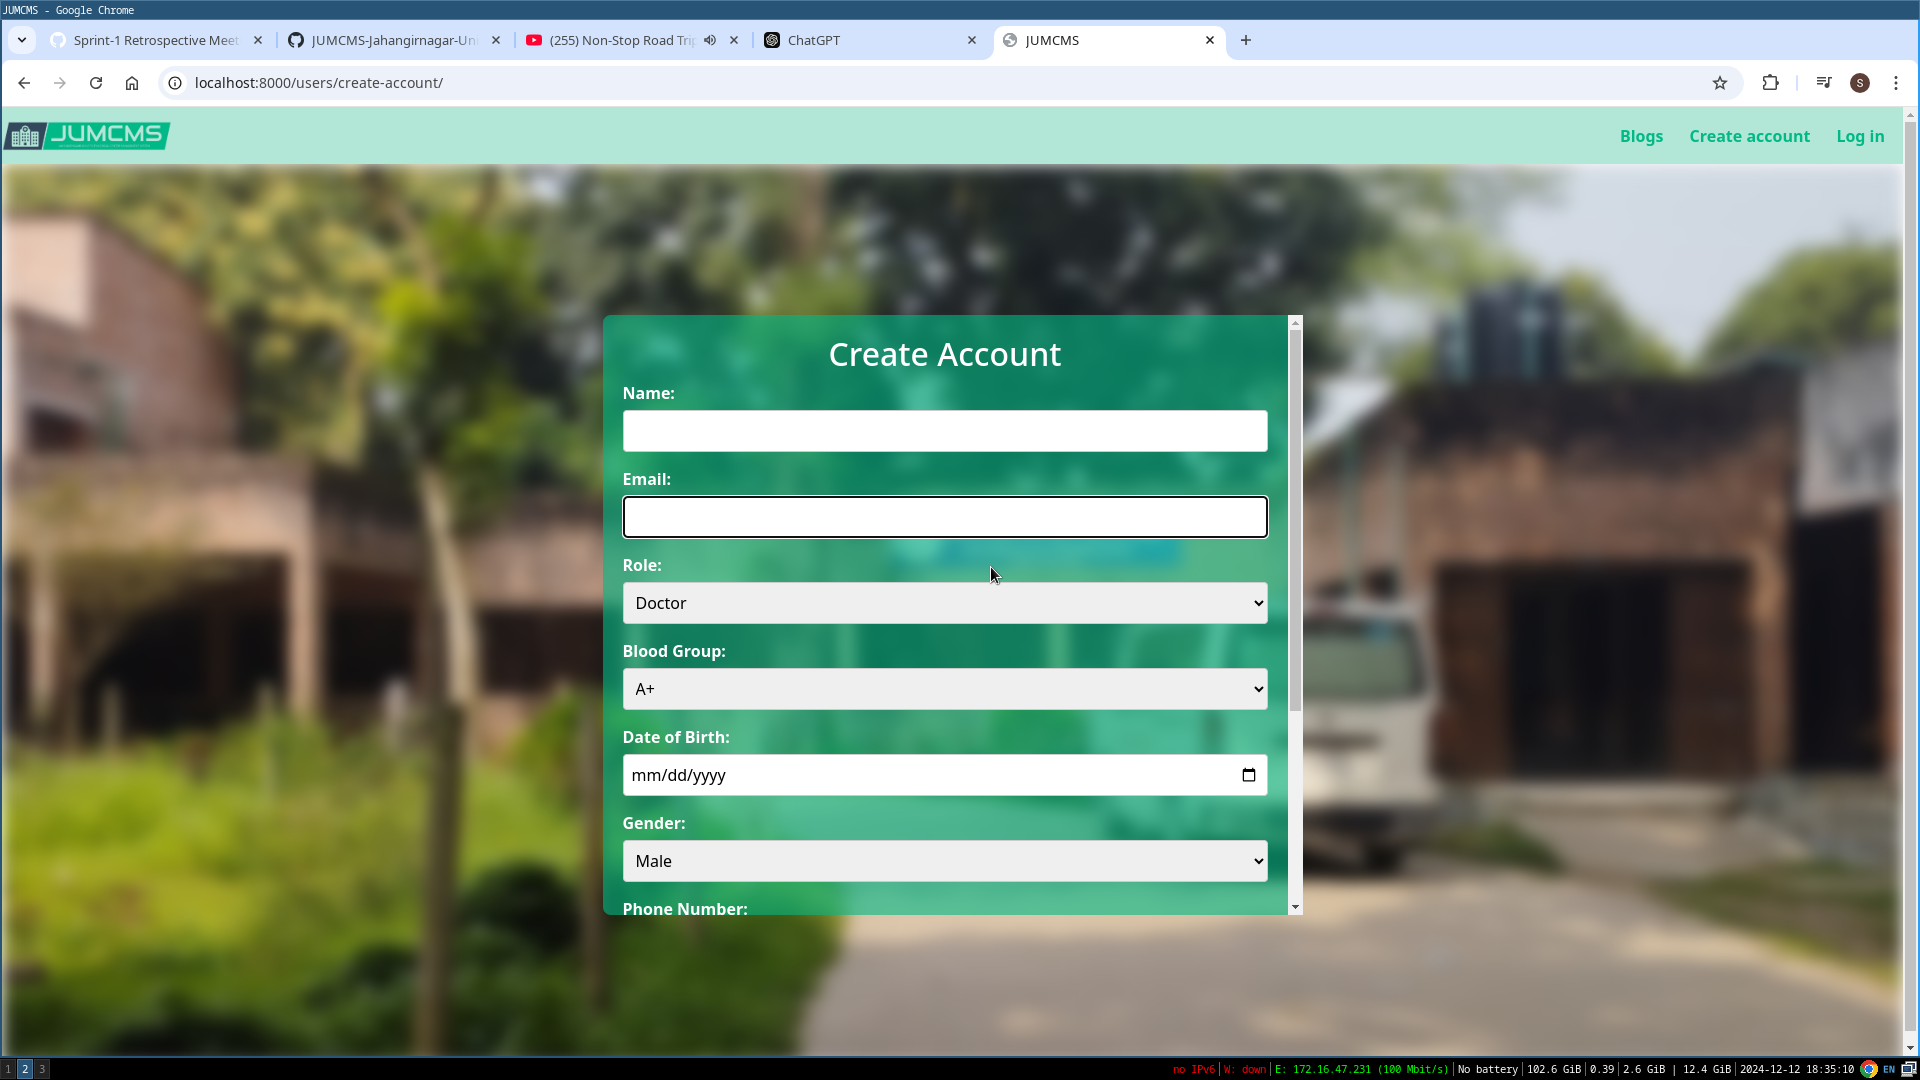
\includegraphics[width=1\textwidth]{images/spr1output2.png}
    \caption{Account Creation form}
    \label{fig:accountcreation}
\end{figure}

\begin{figure}[H]
    \centering
    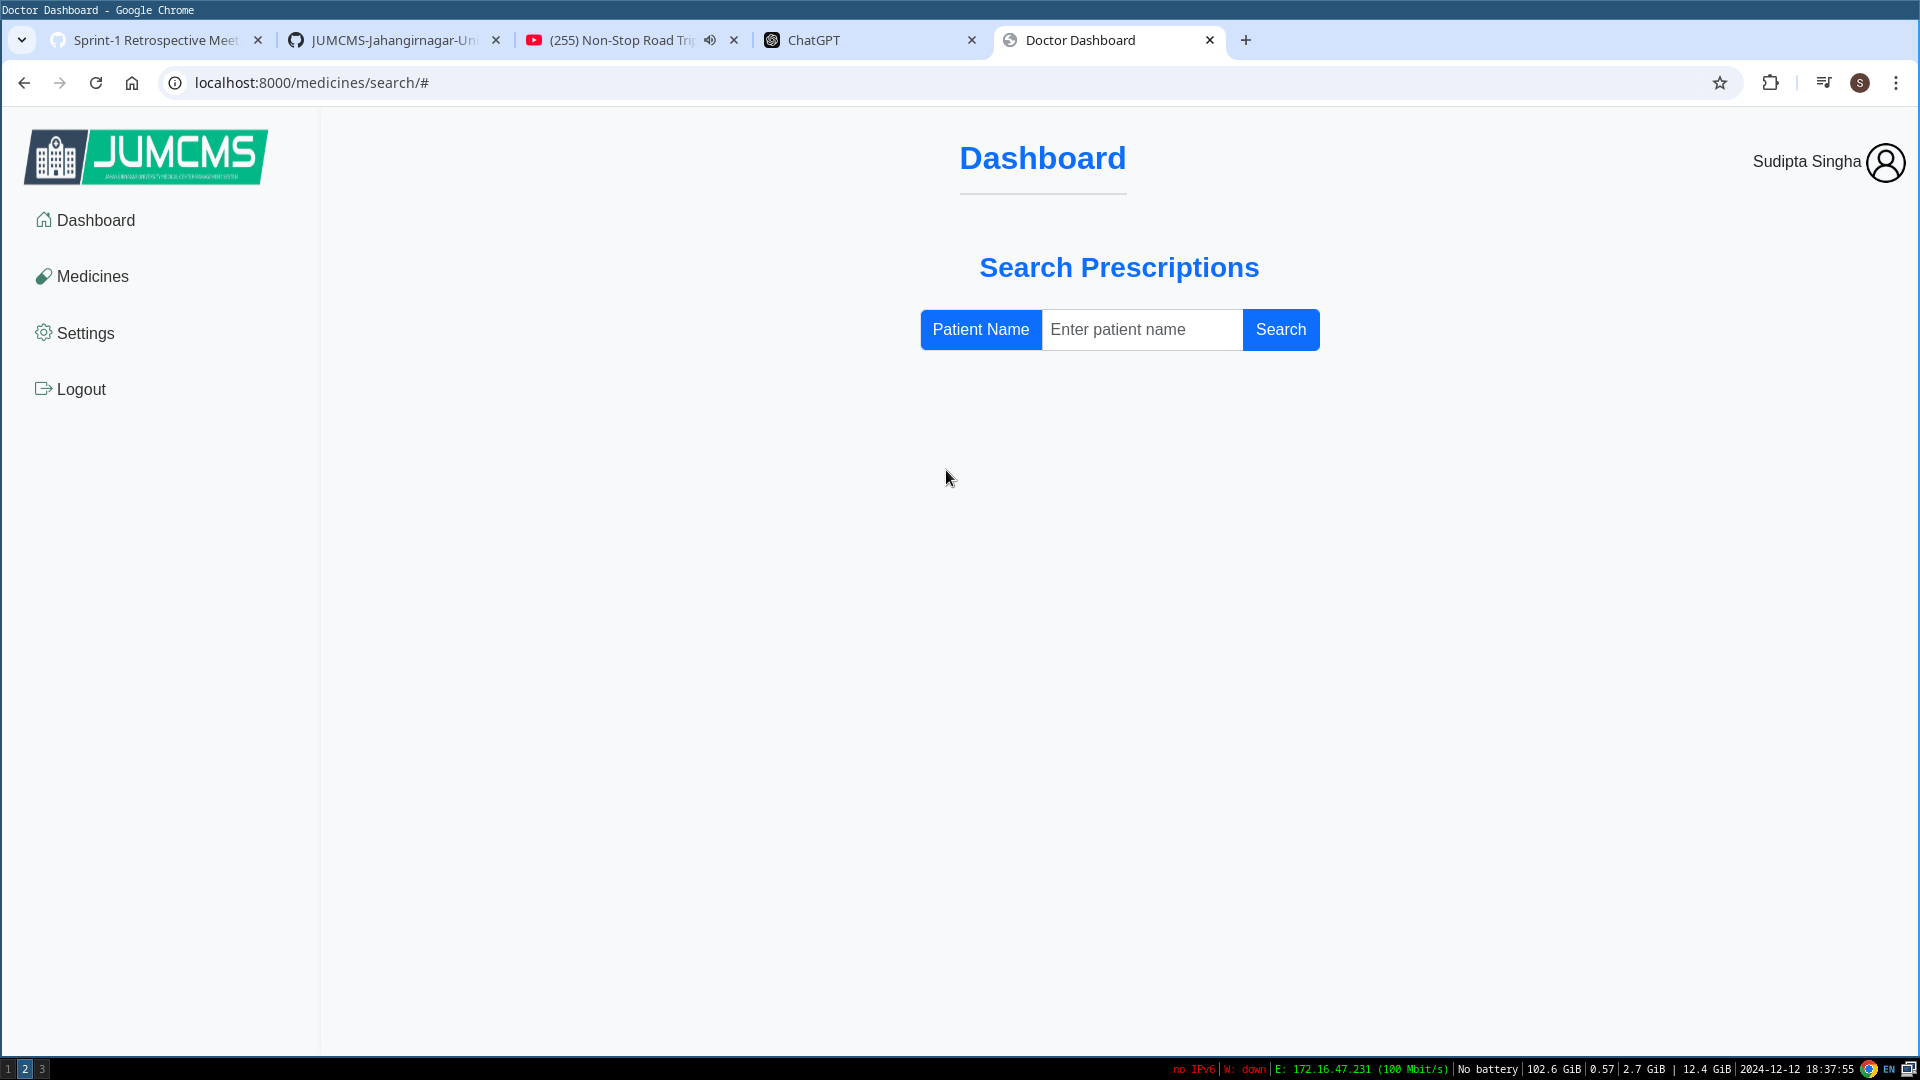
\includegraphics[width=1\textwidth]{images/spr1output3.png}
    \caption{Storekeeper Dashboard}
    \label{fig:storekeeperdashboard}
\end{figure}

\begin{figure}[H]
    \centering
    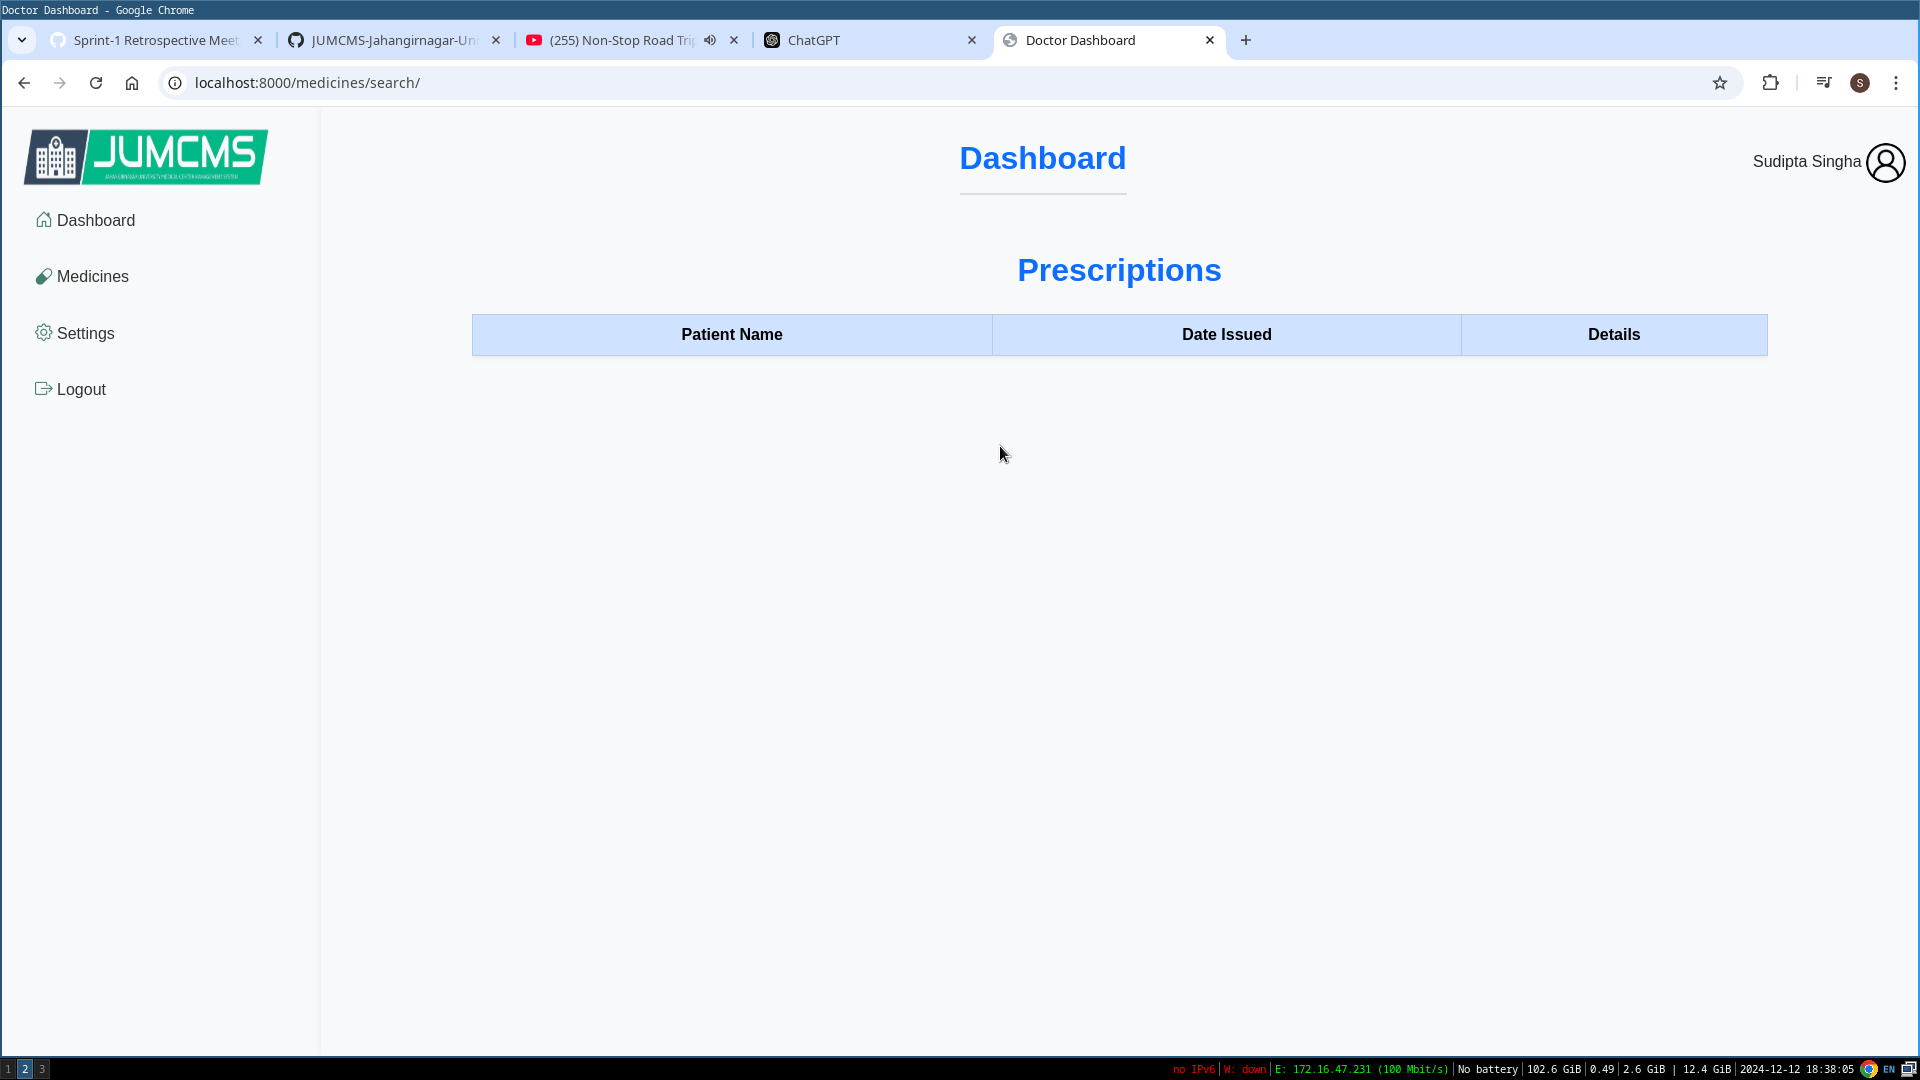
\includegraphics[width=1\textwidth]{images/spr1output4.png}
    \caption{Prescription List}
    \label{fig:prescriptionlist}
\end{figure}
\begin{figure}[H]
    \centering
    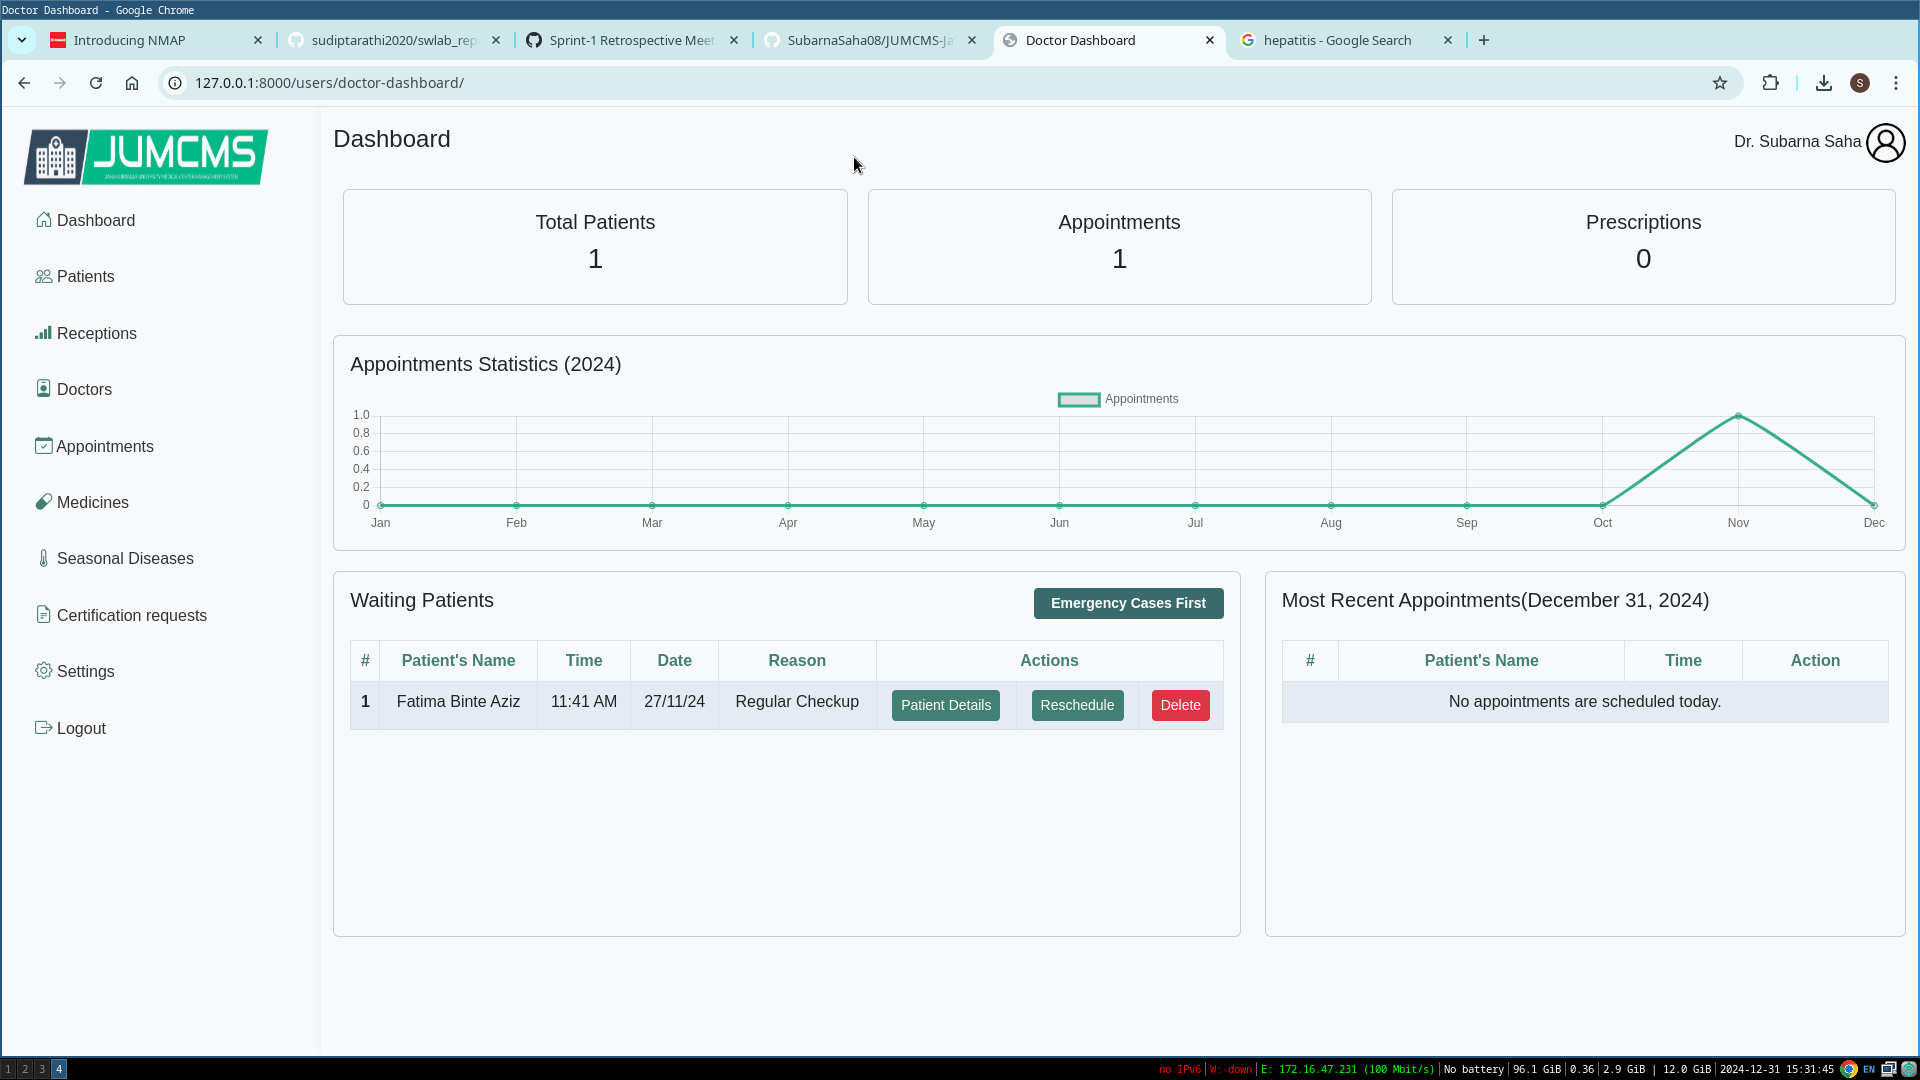
\includegraphics[width=1\textwidth]{images/sprintoutput01.png}
    \caption{Doctor Dashboard}
    \label{fig:doctordashboard}
\end{figure}

\begin{figure}[H]
    \centering
    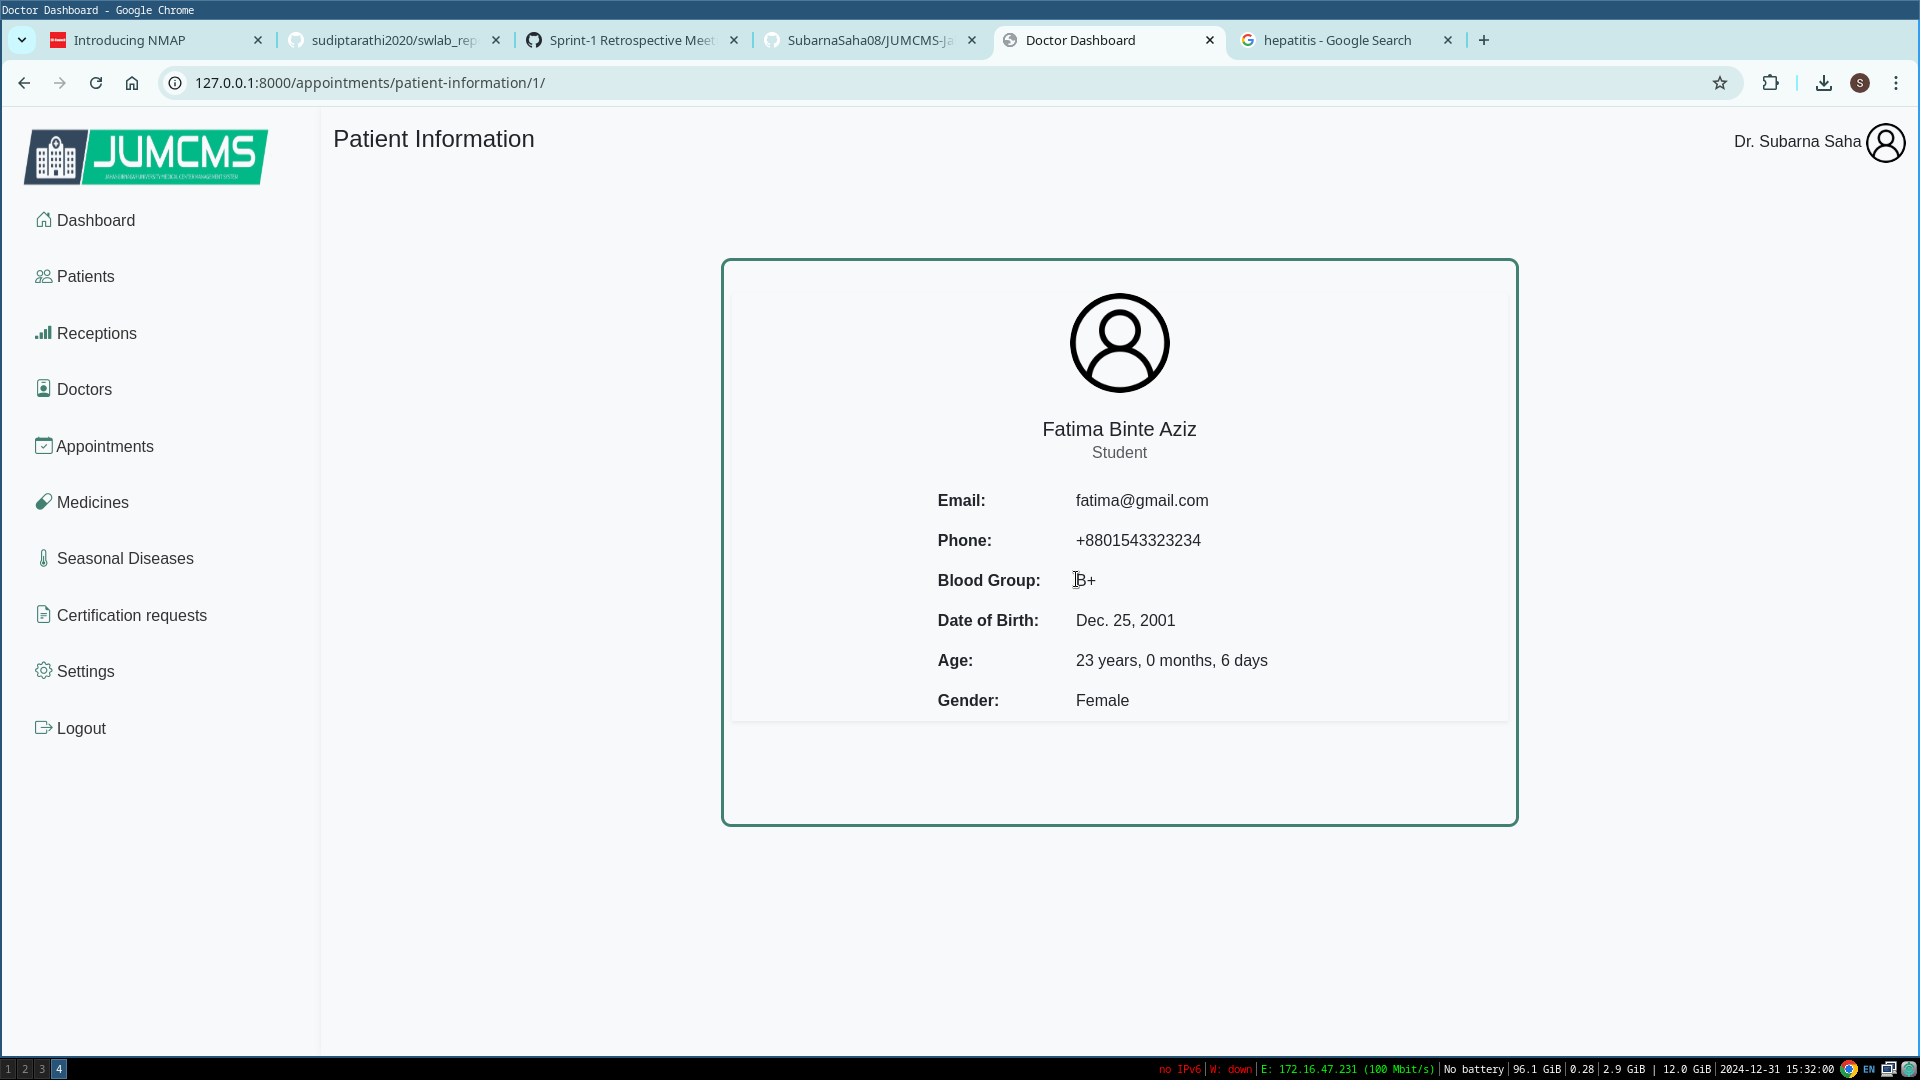
\includegraphics[width=1\textwidth]{images/sprintoutput02.png}
    \caption{Patient Details}
    \label{fig:patientdetails}
\end{figure}

\begin{figure}[H]
    \centering
    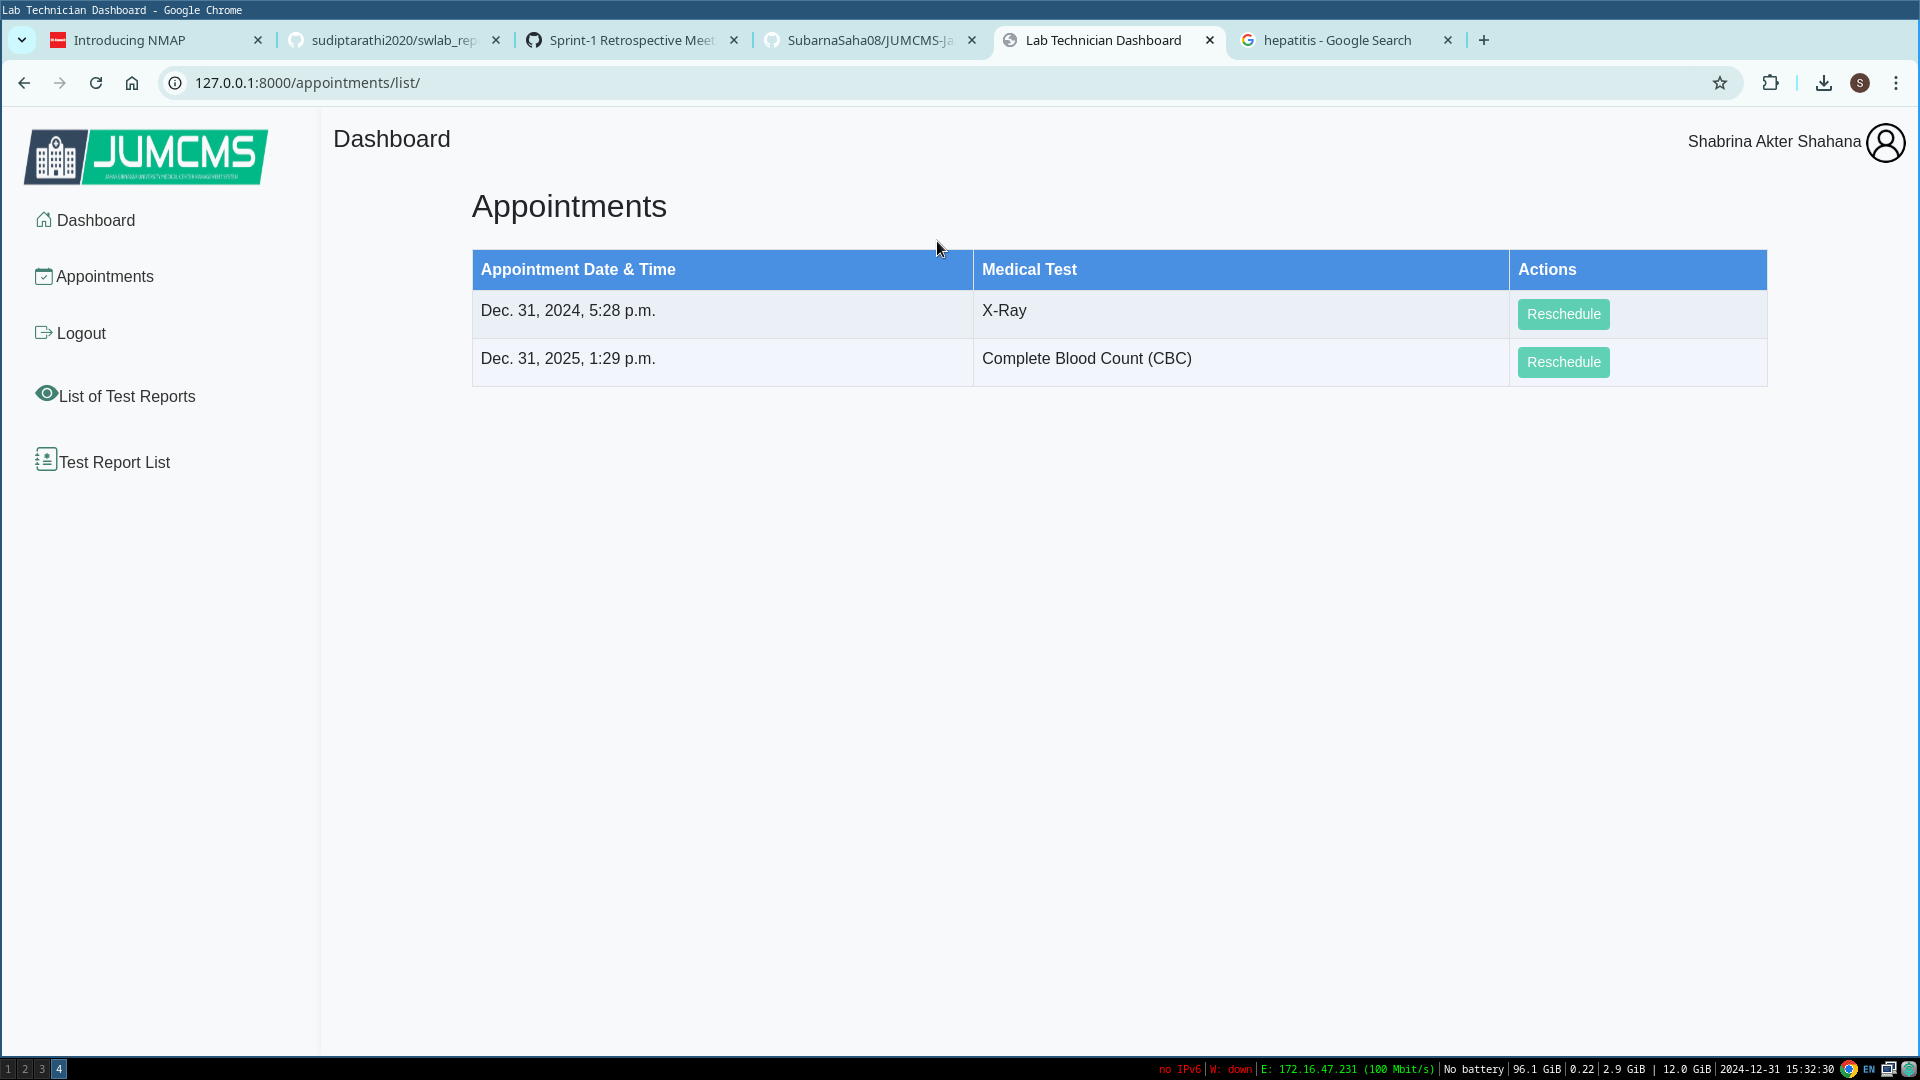
\includegraphics[width=1\textwidth]{images/sprintoutput03.png}
    \caption{Lab Technician Dashboard}
    \label{fig:labtechniciandashboard}
\end{figure}

\begin{figure}[H]
    \centering
    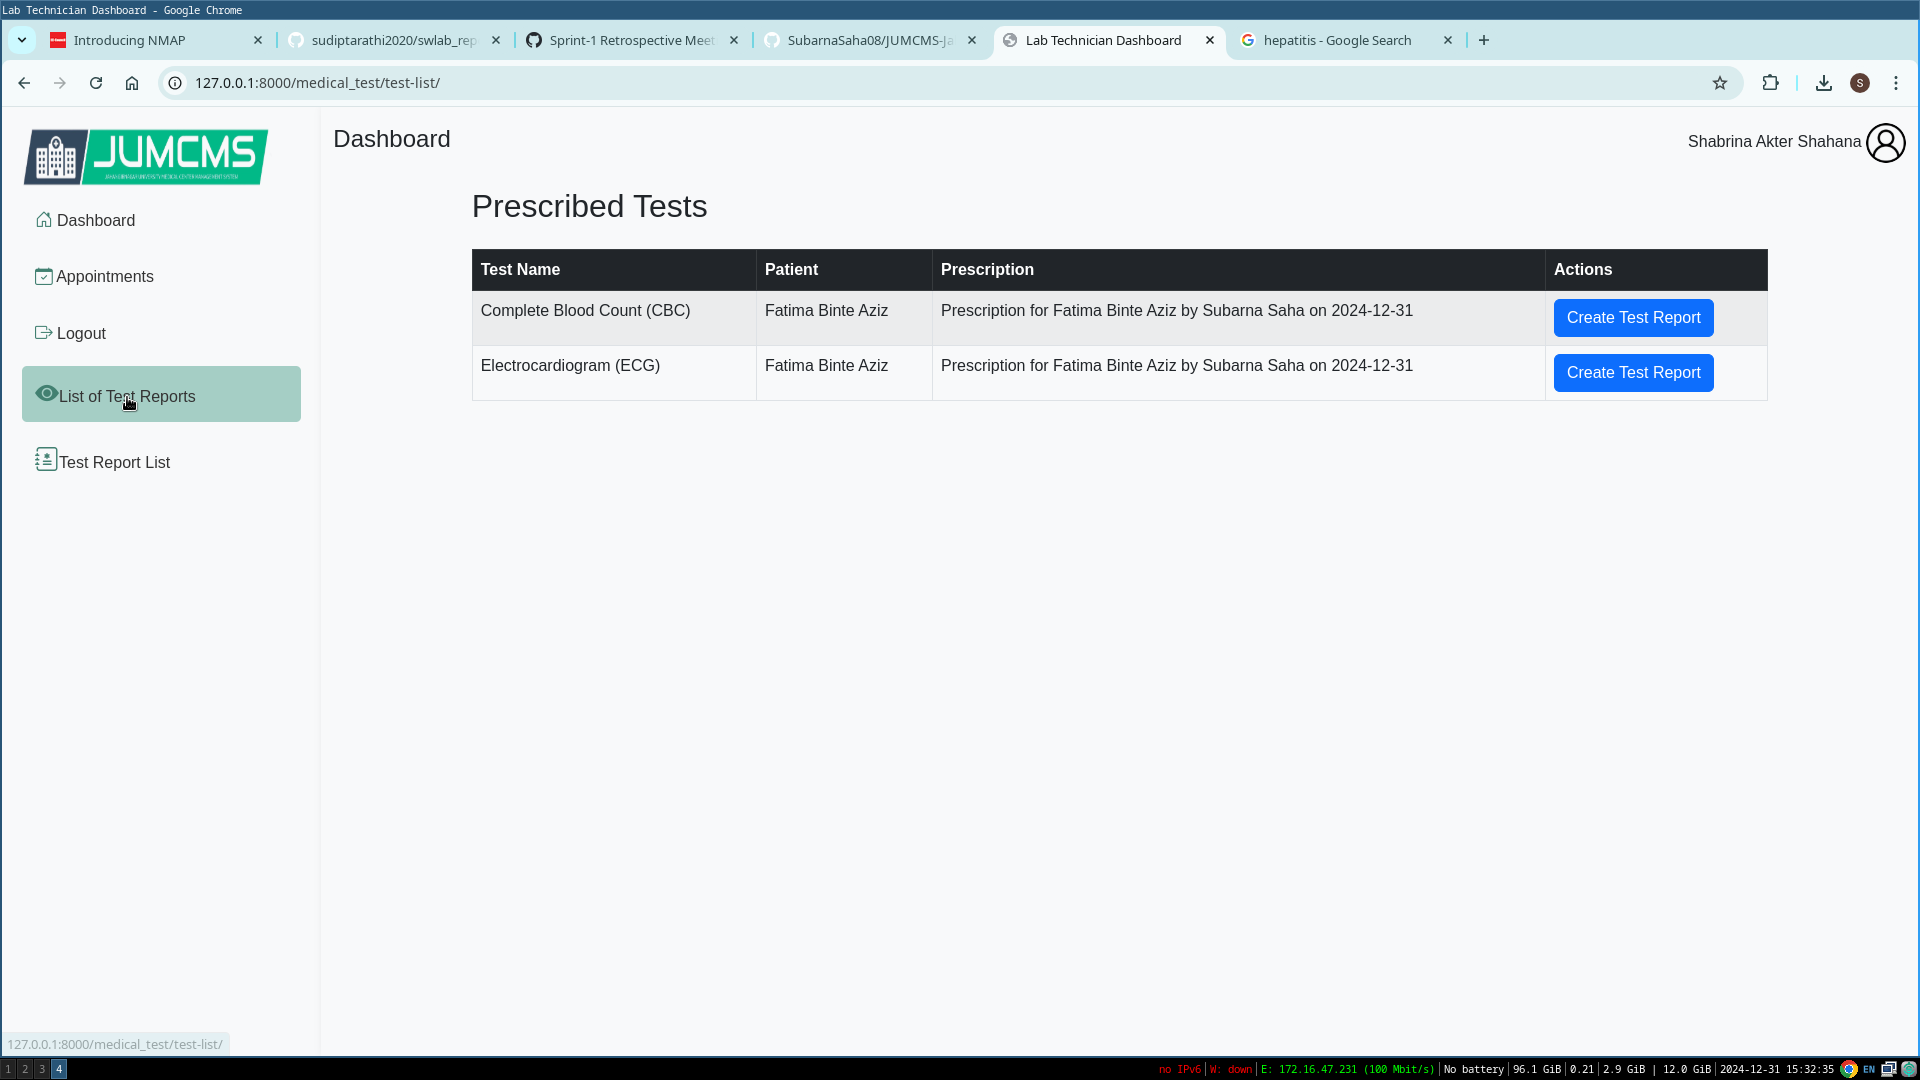
\includegraphics[width=1\textwidth]{images/sprintoutput05.png}
    \caption{Test Report Creation}
    \label{fig:reportcreation}
\end{figure}

\begin{figure}[H]
    \centering
    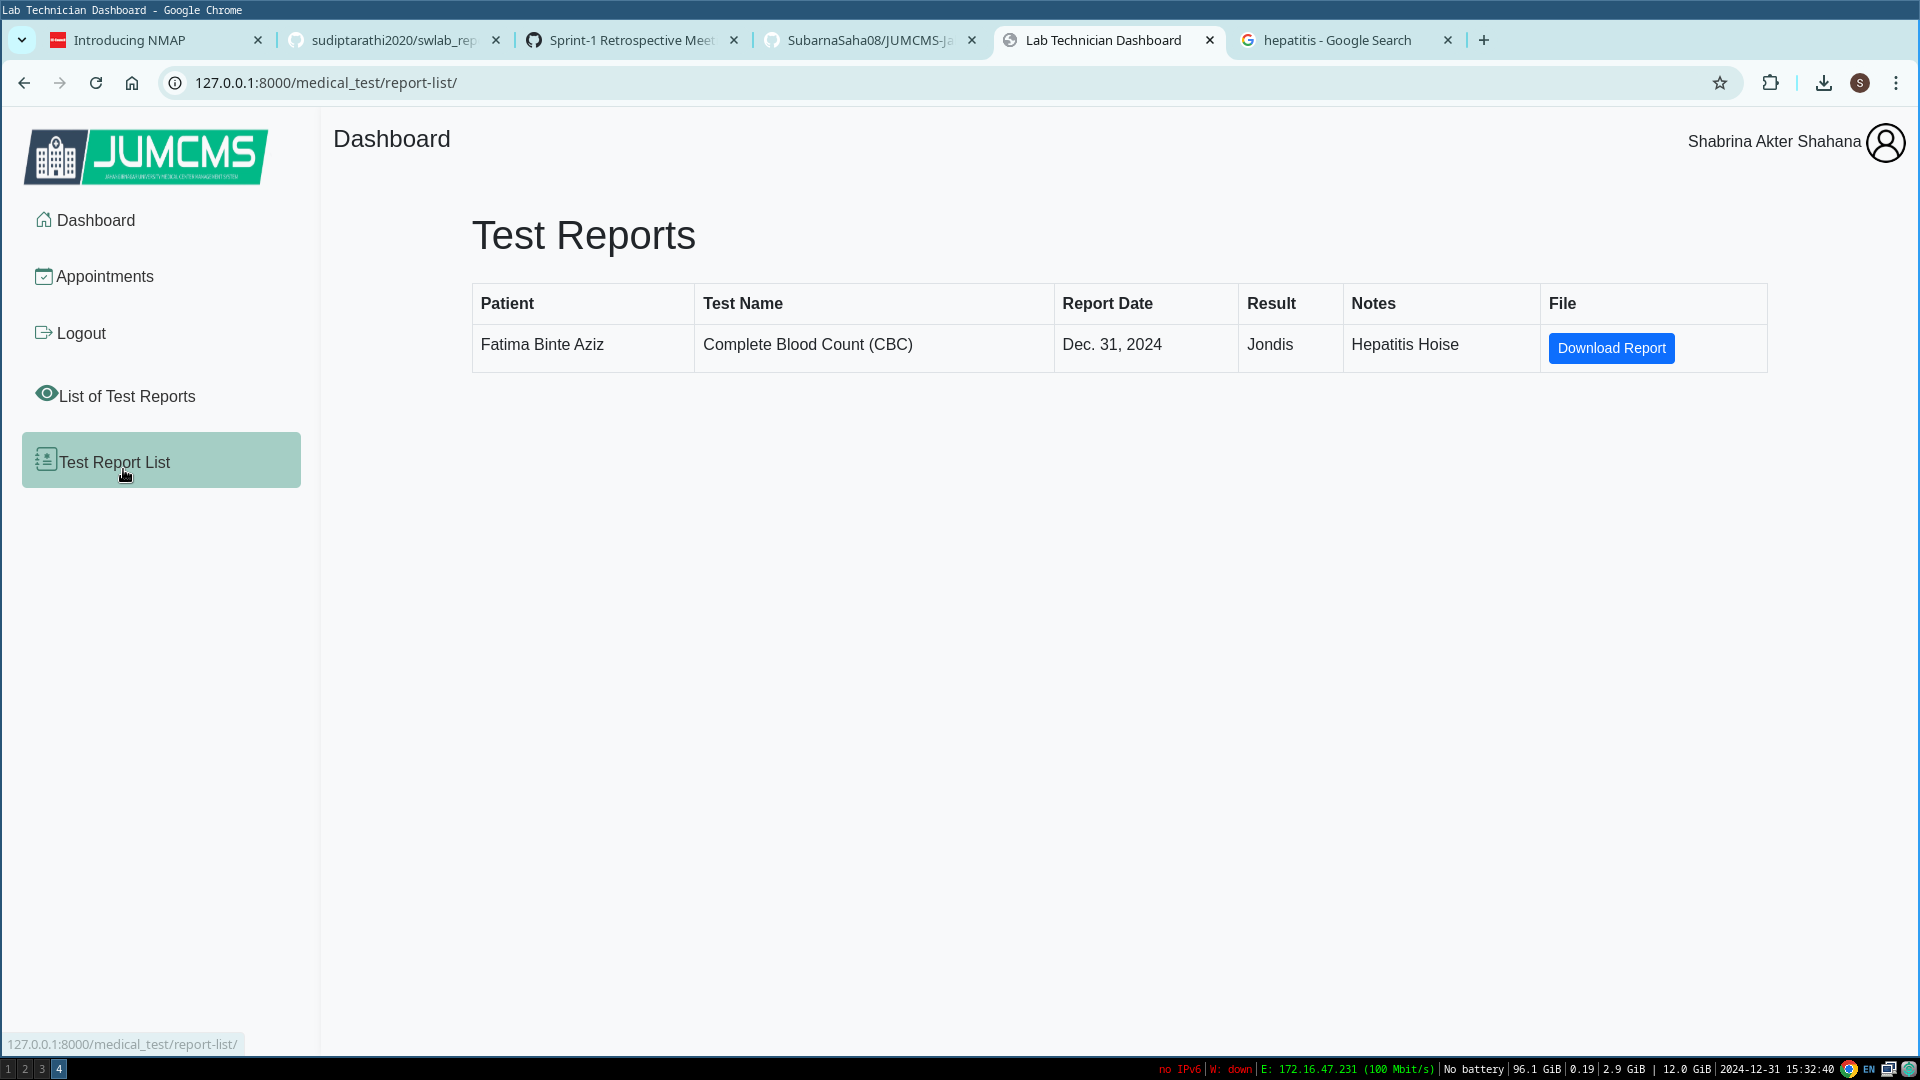
\includegraphics[width=1\textwidth]{images/sprintoutput06.png}
    \caption{List of Reports}
    \label{fig:reportlist}
\end{figure}

\begin{figure}[H]
    \centering
    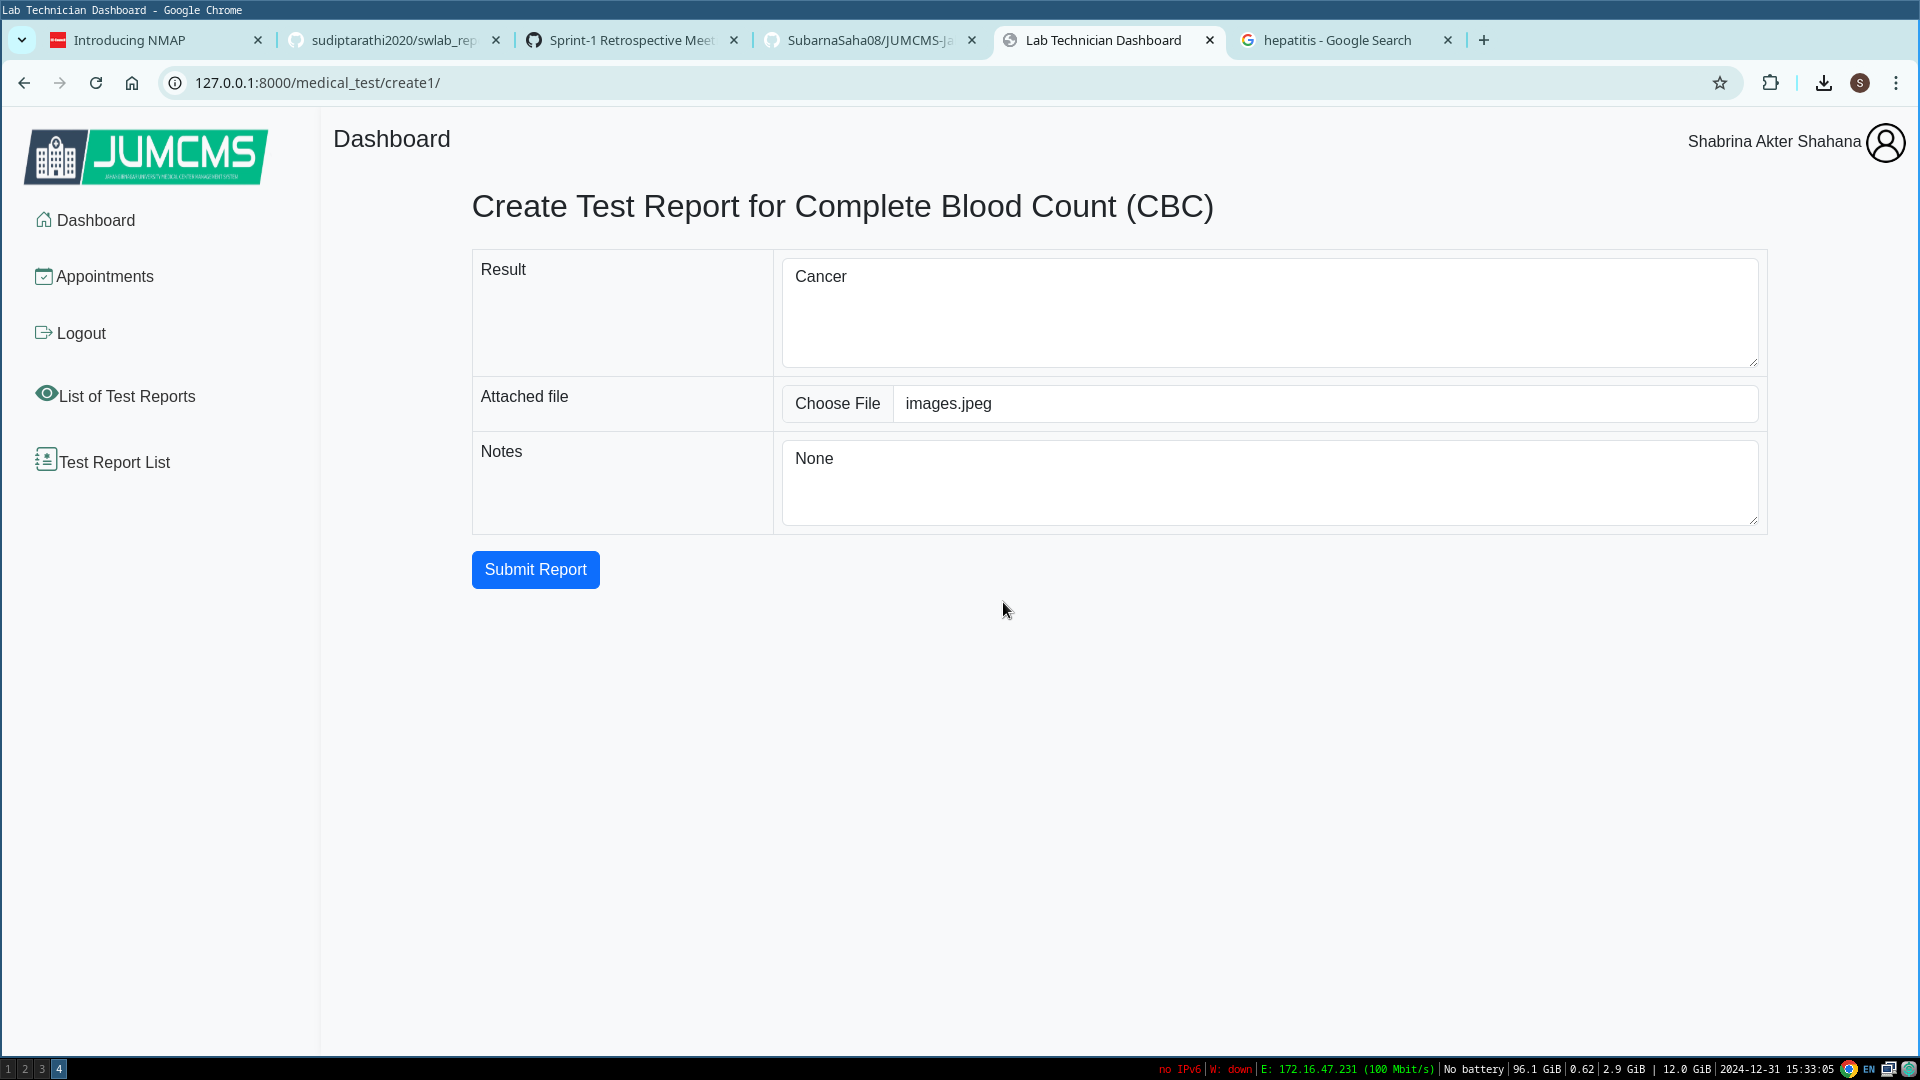
\includegraphics[width=1\textwidth]{images/sprintoutput07.png}
    \caption{Report Creation Form}
    \label{fig:reportform}
\end{figure}

\begin{figure}[H]
    \centering
    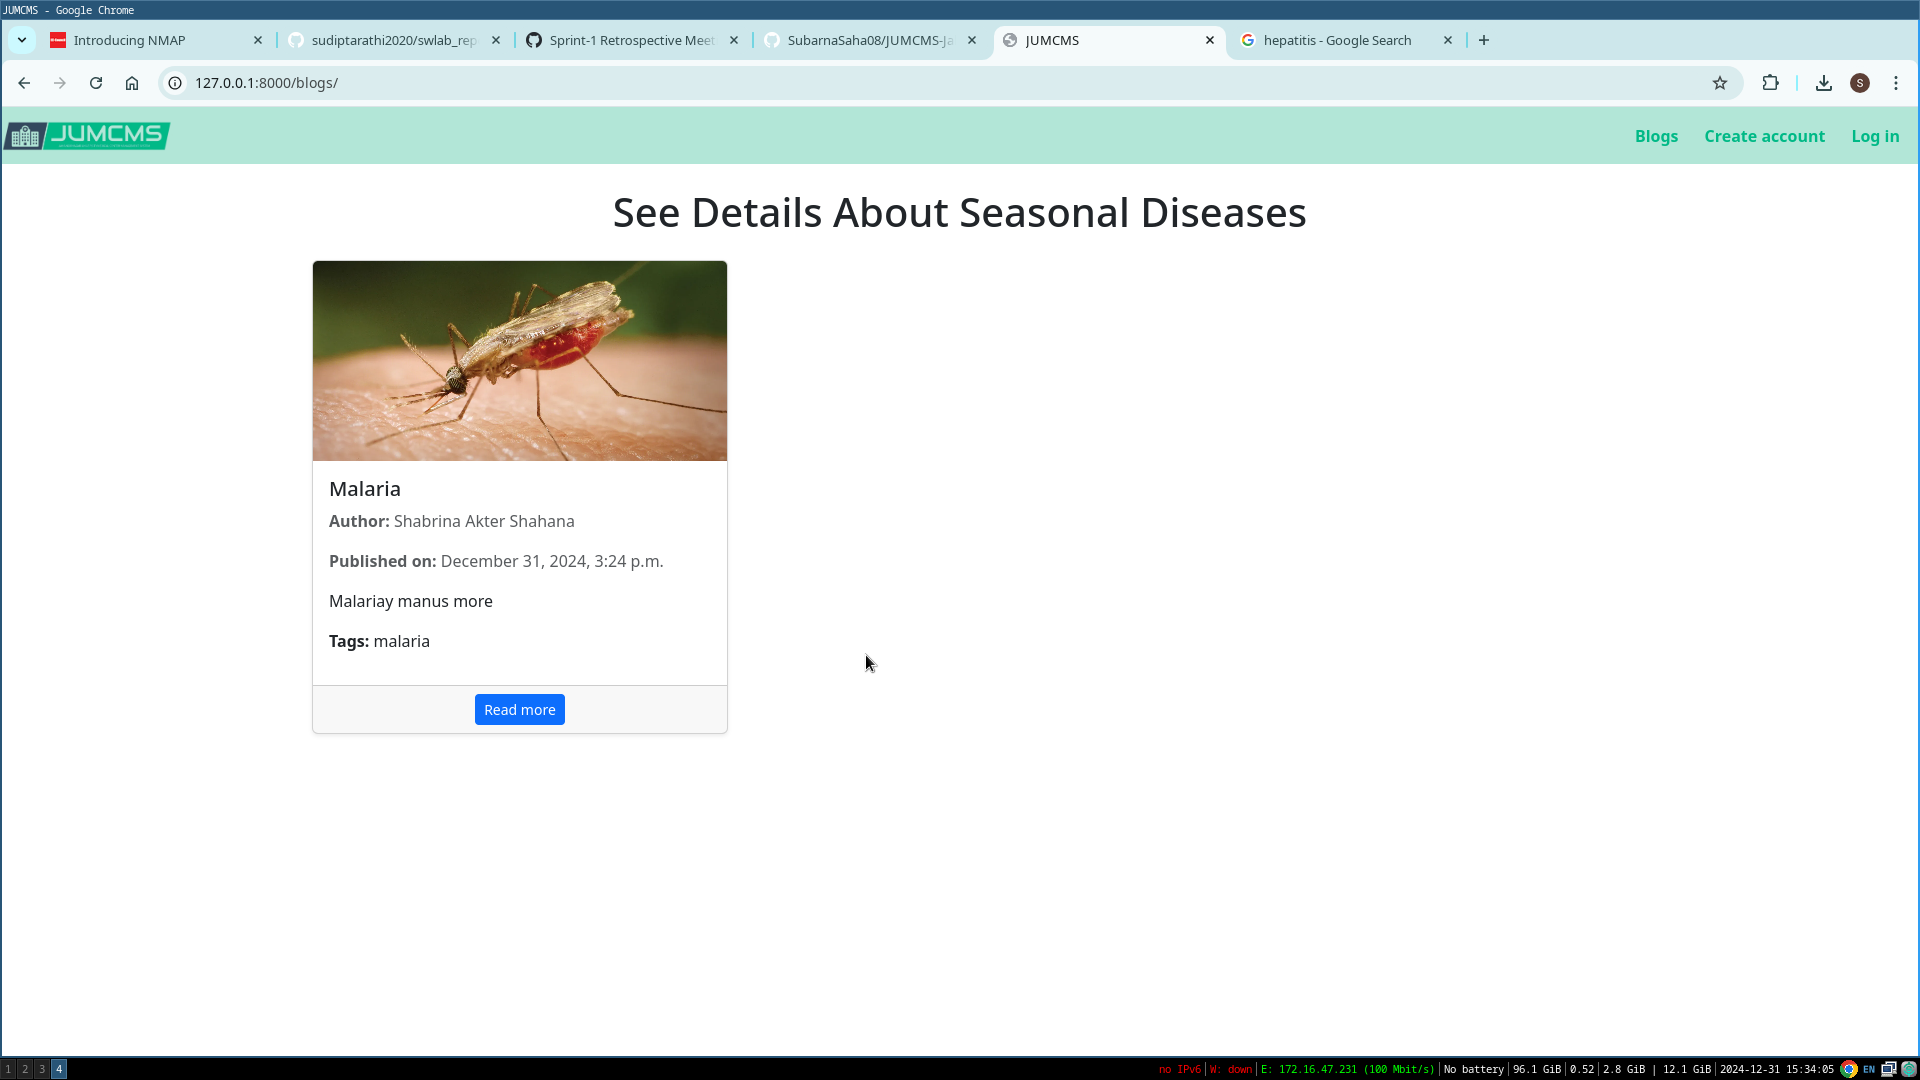
\includegraphics[width=1\textwidth]{images/sprintoutput08.png}
    \caption{Blogs}
    \label{fig:blogs}
\end{figure}

\begin{figure}[H]
    \centering
    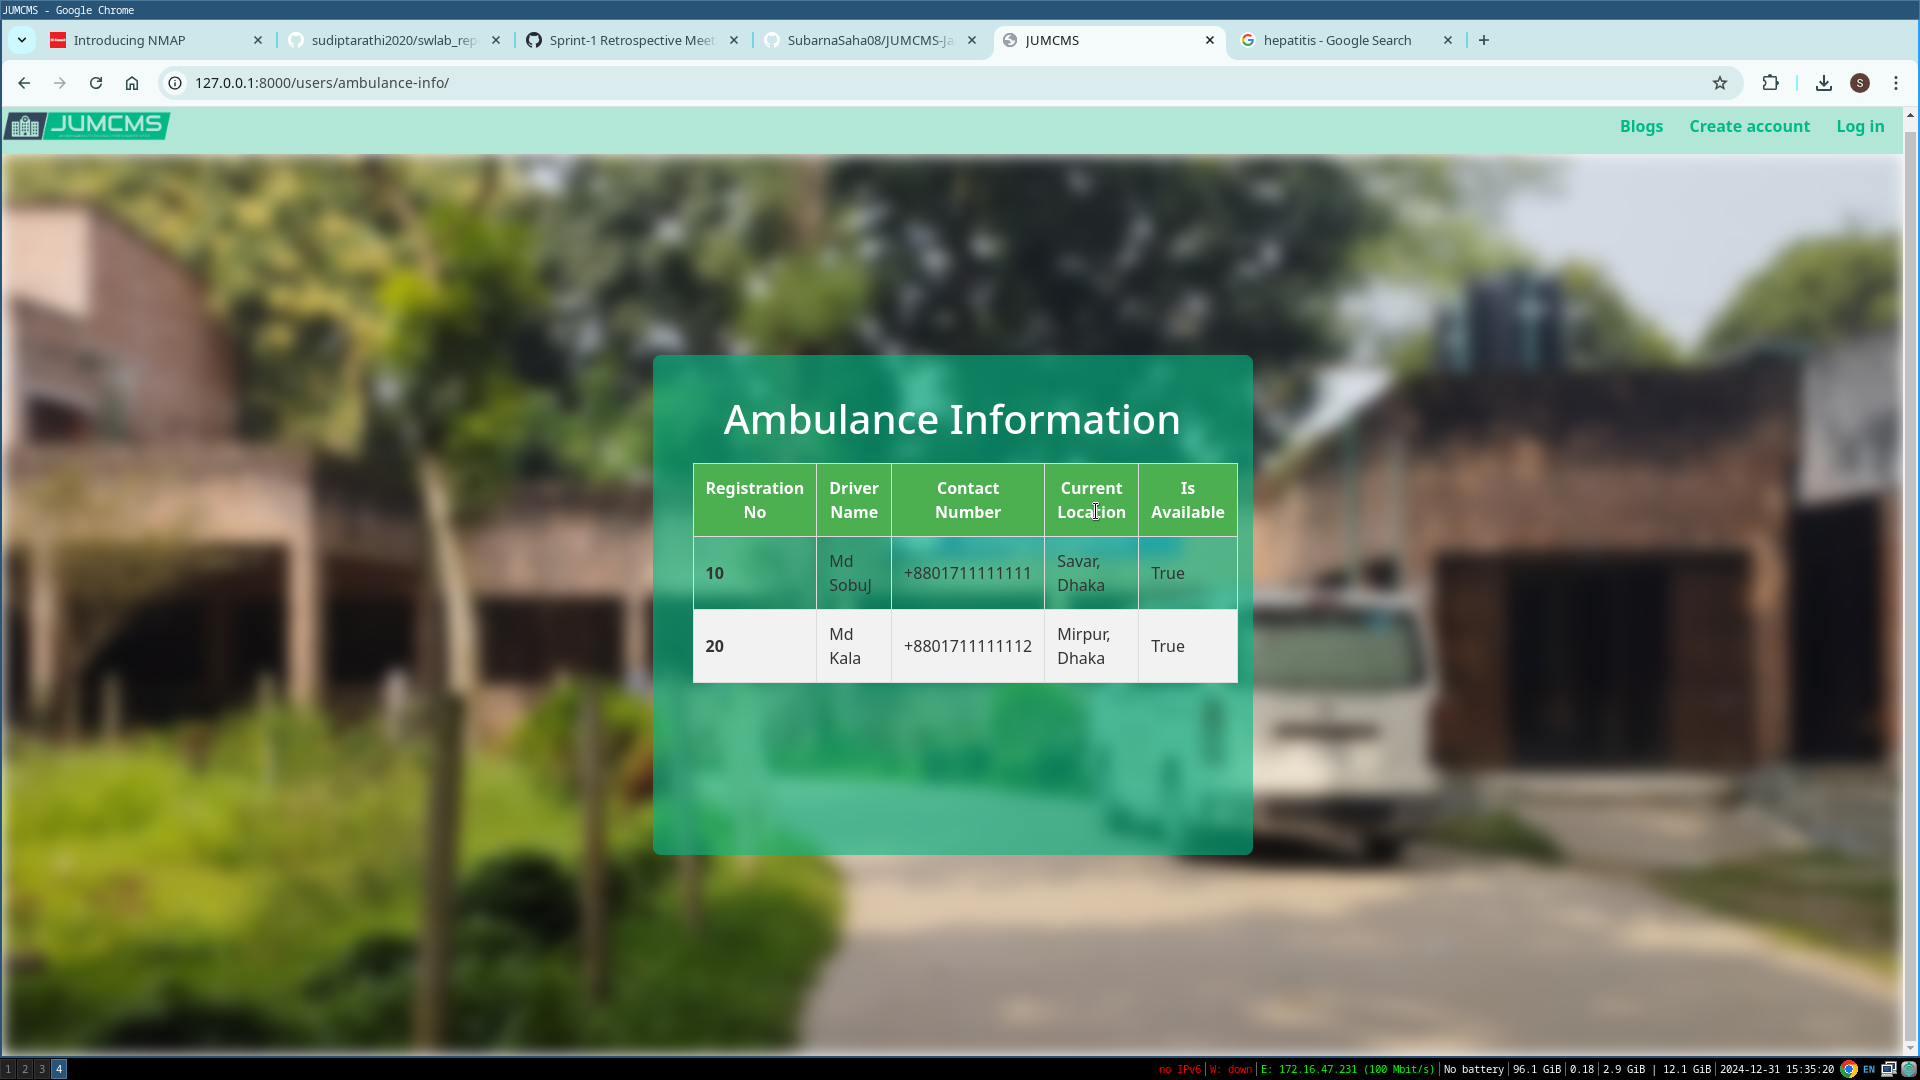
\includegraphics[width=1\textwidth]{images/sprintoutput09.png}
    \caption{Drivers information}
    \label{fig:driverinformation}
\end{figure}

\newpage
\section{Sprint Retrospective}
\subsection{What Went Well}
Discussing the positive aspects of the sprint, including achievements, successful teamwork, and processes that worked well.
\begin{itemize}
    \item Role-based Login functionality was completed successfully where custom tests are passed.
    \item Implementation of features of displaying different attributes of a Doctor in a user-friendly went smoothly and finished testing the features.
    \item The Make Appointment feature was successfully implemented, allowing users to schedule appointments with doctors as required.
    \item The Create Blogpost feature was successfully developed and integrated into the project, meeting all the initial requirements. Testing and debugging were managed well, leading to a relatively smooth development process.
    \item Completed Account Creation feature.
    \item Completed Dispense Medicine feature where custom tests are passed for all feature.
    \item Implementation of text appointment rescheduling functionalities went well.
    \item Completed View Ambulance Information feature and implemented User Interface for viewing ambulance information in tabular format.
    \item The team collaborated effectively, with each member contributing efficiently to their assigned tasks.
\end{itemize}
\subsection{What Could Be Improved}
Identifying areas for improvement, including challenges faced, bottlenecks, and aspects of the sprint that could be better.
\begin{itemize}
    \item Problems faced during implementing the reset password option, the password saving feature and
        inactivity detection procedure. These features could be implemented for the better performance of the
        application.
    \item The appointment form could be optimized for better user experience where UI could be more smooth and
        documentation for the feature could be improved.
    \item Sprint planning and time estimation could be improved, documentation could be improved to include
        more detailed steps for setting up the feature and testing coverage for edge cases could be increased,
        especially for image uploads and error handling.
    \item The UI could be improved and more knowledge about URL routing would be helpful for handling
        challenges in URL routing.
    \item Problem faced during implementation as I preferred bottom-up approach like completed the backend
        part first then the frontend which introduced me redundant implementation. Will try to avoid this in
        future sprint.
    \item The User Interface could be improved to show exact location of ambulance in google map.
\end{itemize}
\subsection{Lessons Learned}
Capturing any key lessons learned from the sprint that can be applied to future sprints.
\begin{itemize}
    \item Understood that one needs to be careful while using Toggl as it tracks time based on the local
        device's clock. Any changes to the device's time settings may disrupt the accuracy of Toggl's
        tracking. Gained the idea of how to estimate time for any project.
    \item Learned about Testing and bug fixes.
        Estimated time was too short, we have learned about a good estimated average time.
    \item Got better understanding of Django by actually implementing the product and learned how to use Toggl as a time tracking tool.
    \item Should follow the conventional approaches while implementation and will have to be more careful about using Toggl as once I forgot to stop the Toggl which made a real mess-up in tracking.
    \item How to use Django \& HTML for development and toggl for time tracking. 
\end{itemize}
\newpage
\section{Activity Log}
My contribution During Sprint 1:
\subsection{Scrum Meeting Update 1}
\begin{itemize}
    \item Completed the coding for role-based registration of the JUMCMS.
    \item Prepared unit tests for the Create account part.
\end{itemize}
\begin{figure}[H]
    \centering
    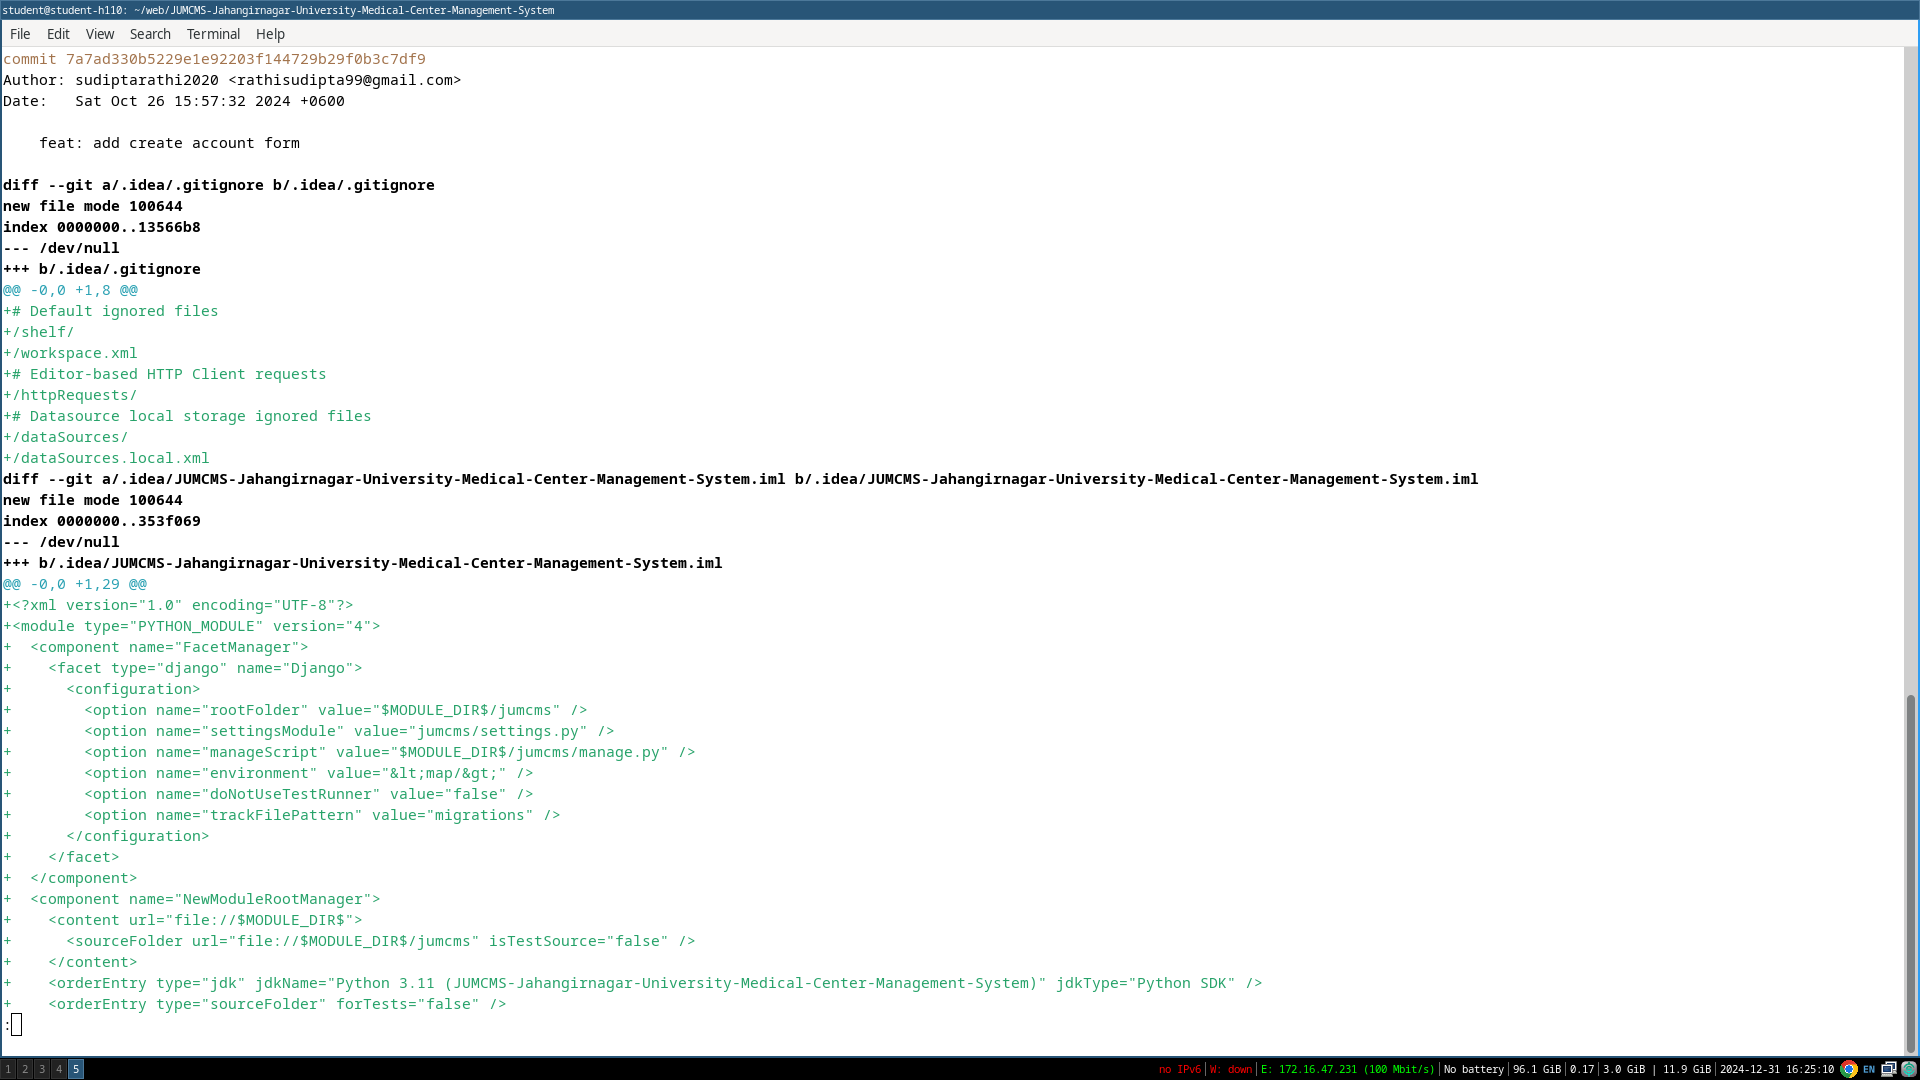
\includegraphics[width=1\textwidth]{images/scr1out1.png}
    \caption{Git log for Create Account feature}
    \label{fig:gitlogcreateaccount}
\end{figure}

\begin{figure}[H]
    \centering
    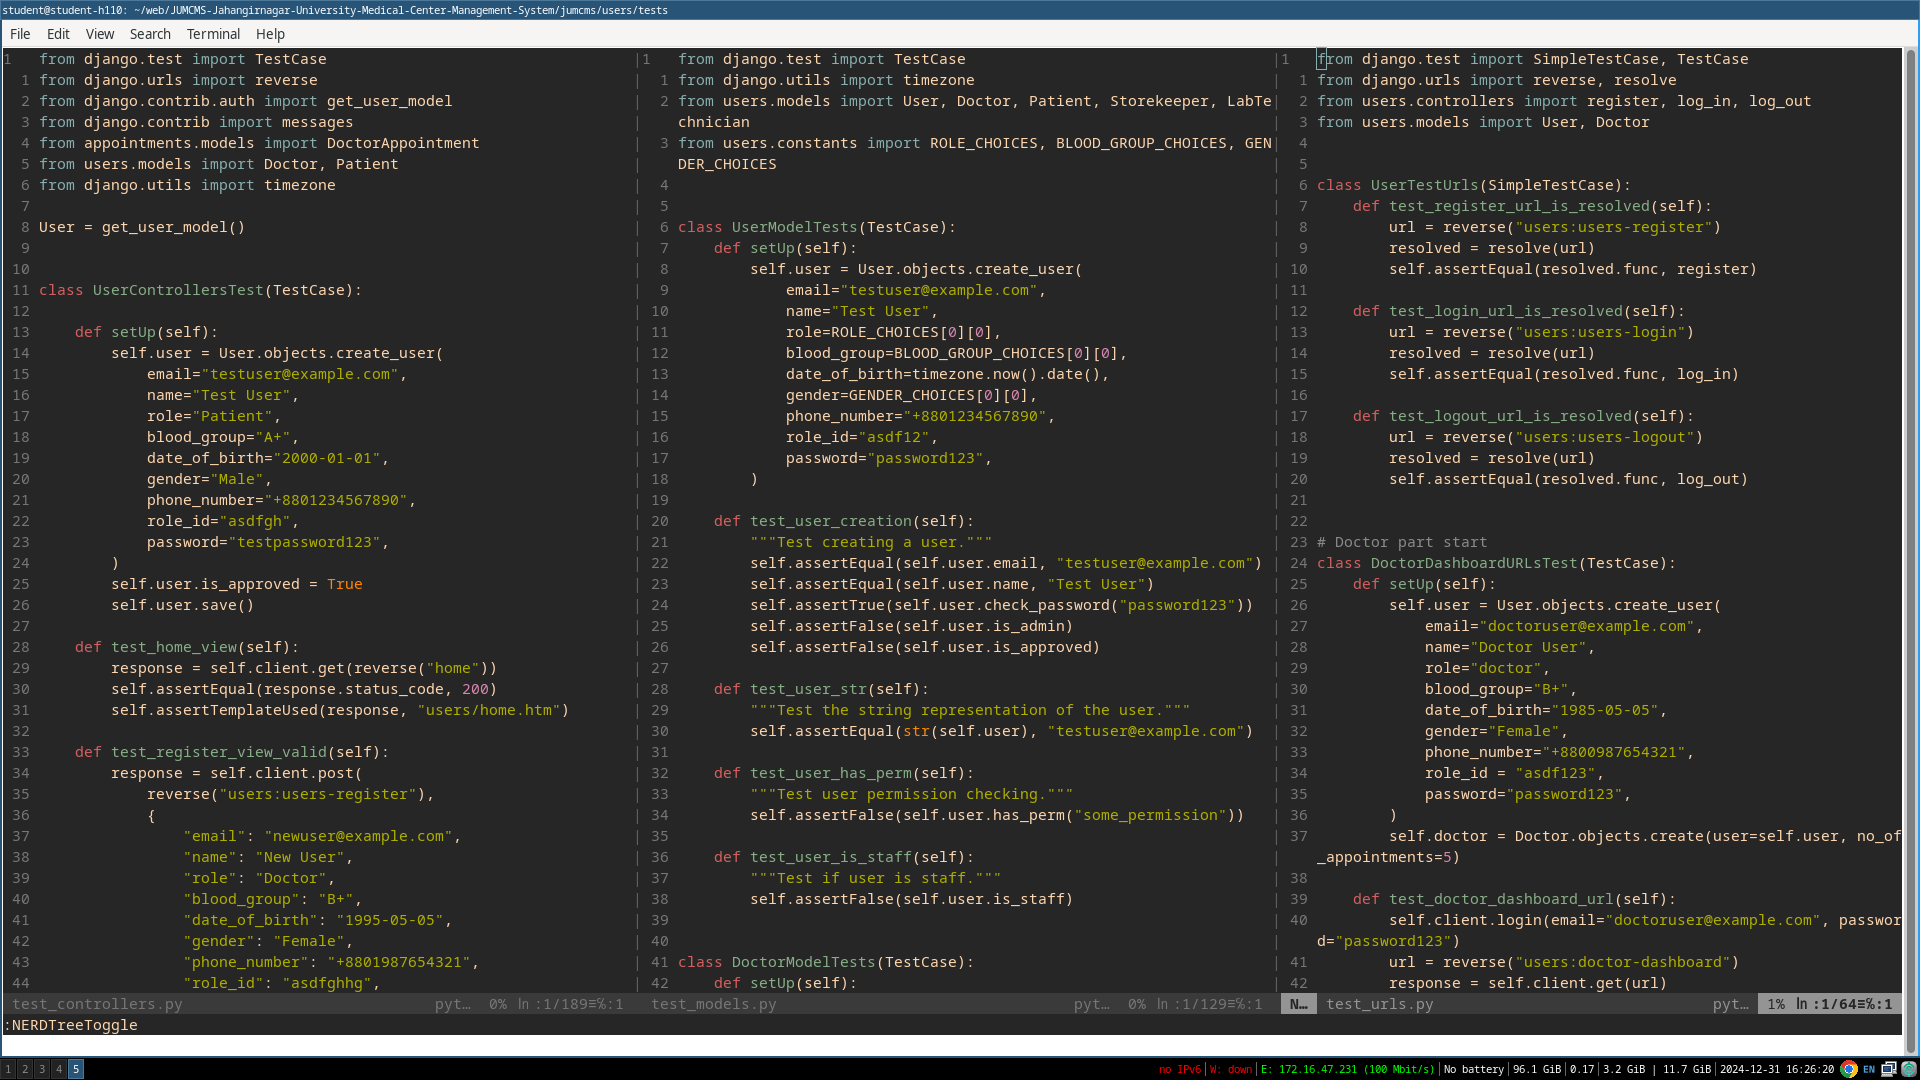
\includegraphics[width=1\textwidth]{images/scr1out2.png}
    \caption{Test case and test file for create account and login}
    \label{fig:testcreateaccount}
\end{figure}



\subsection{Scrum Meeting Update 2}
\begin{itemize}
    \item Designed Store-manager dashboard.
\end{itemize}

\begin{figure}[H]
    \centering
    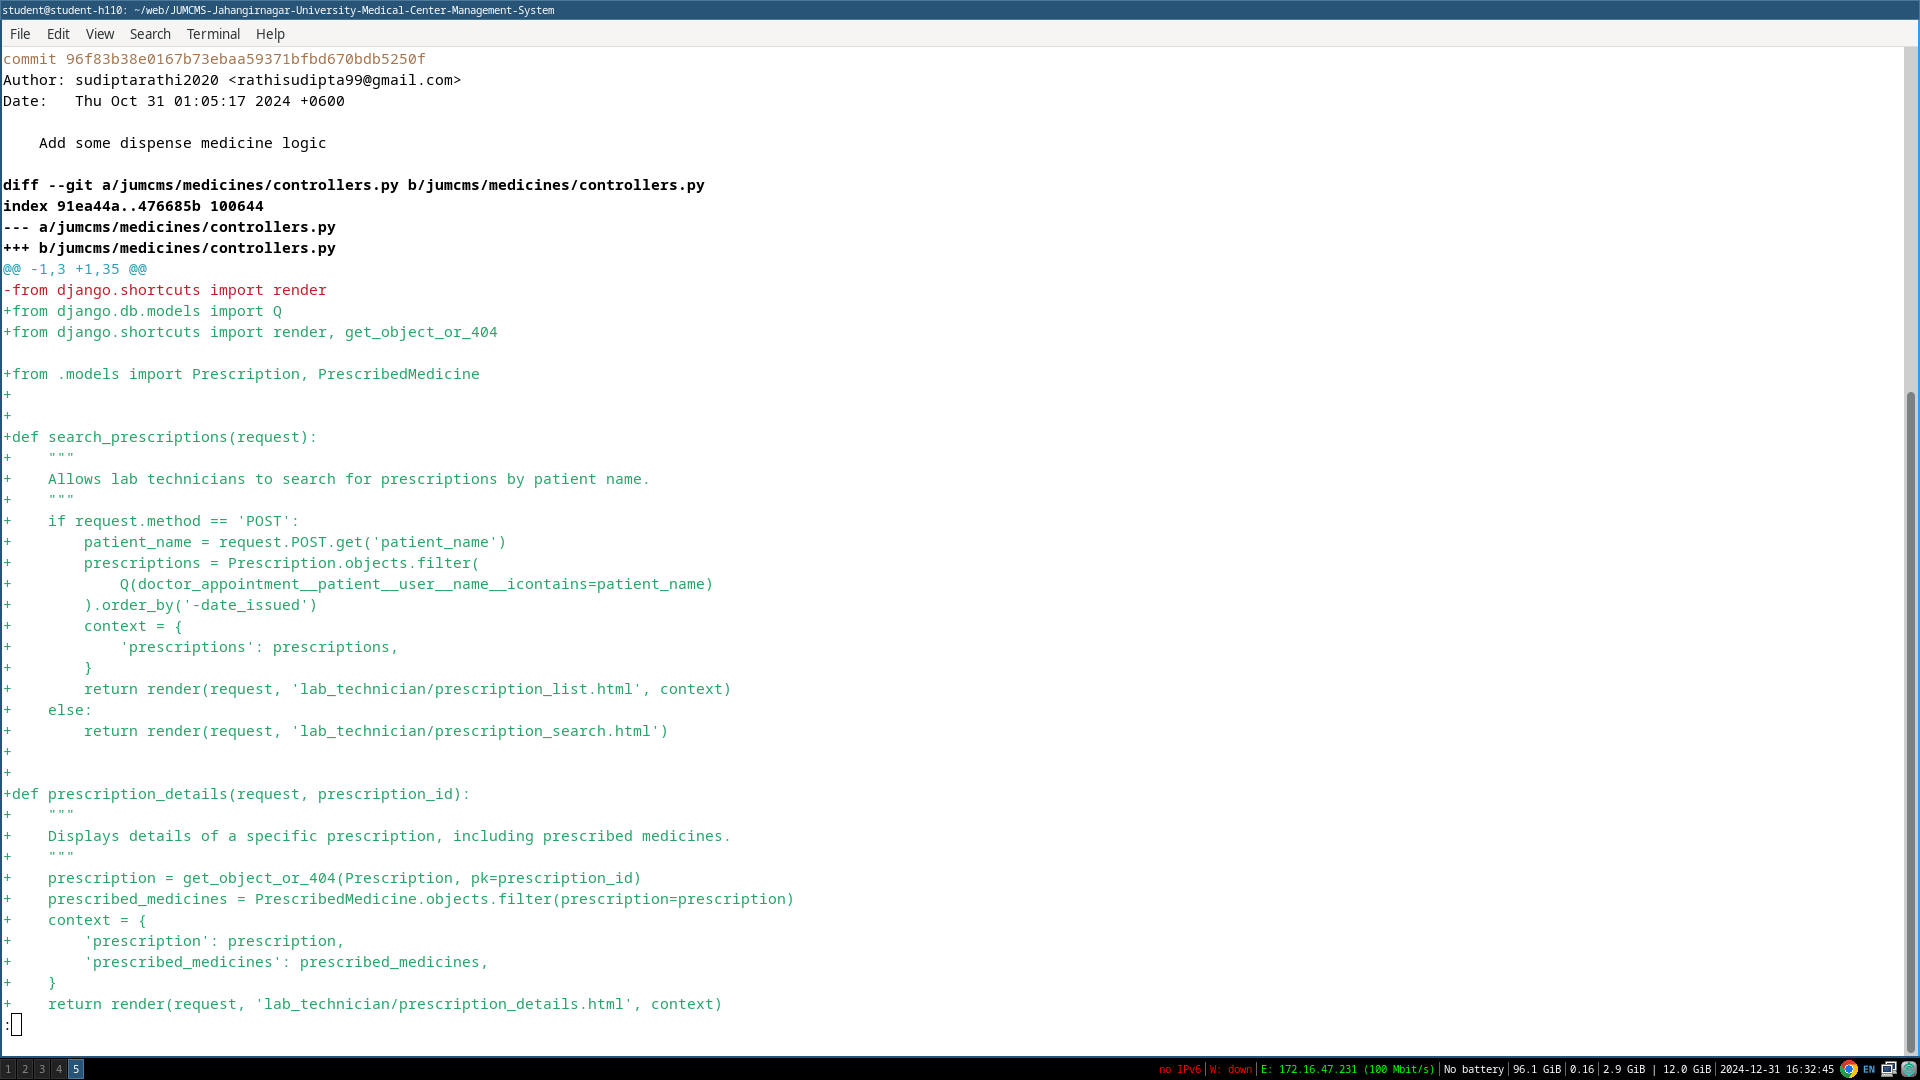
\includegraphics[width=1\textwidth]{images/scr2git1.png}
    \caption{Git log for dispense medicine logic}
    \label{fig:gitlogscr21}
\end{figure}

\begin{figure}[H]
    \centering
    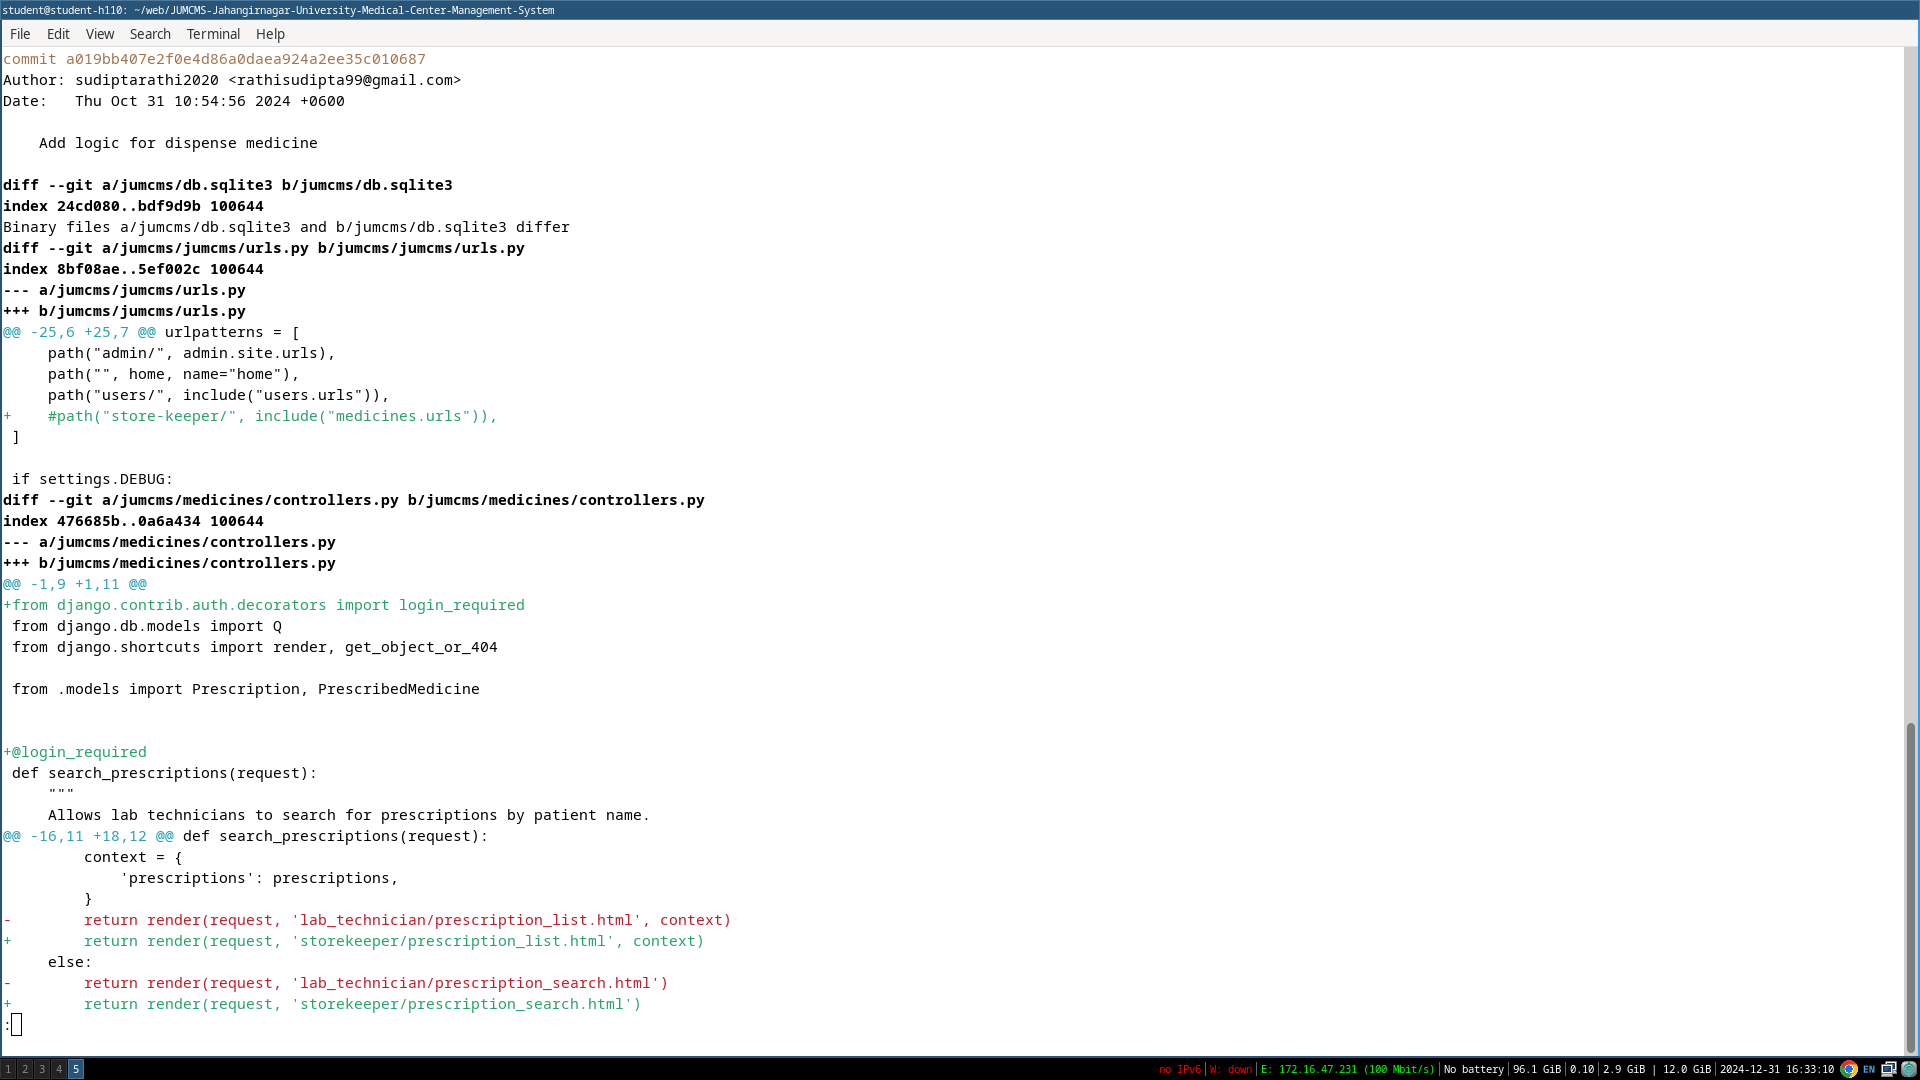
\includegraphics[width=1\textwidth]{images/scr2git2.png}
    \caption{Git log for dispense medicine logic}
    \label{fig:gitlogscr22}
\end{figure}


\begin{figure}[H]
    \centering
    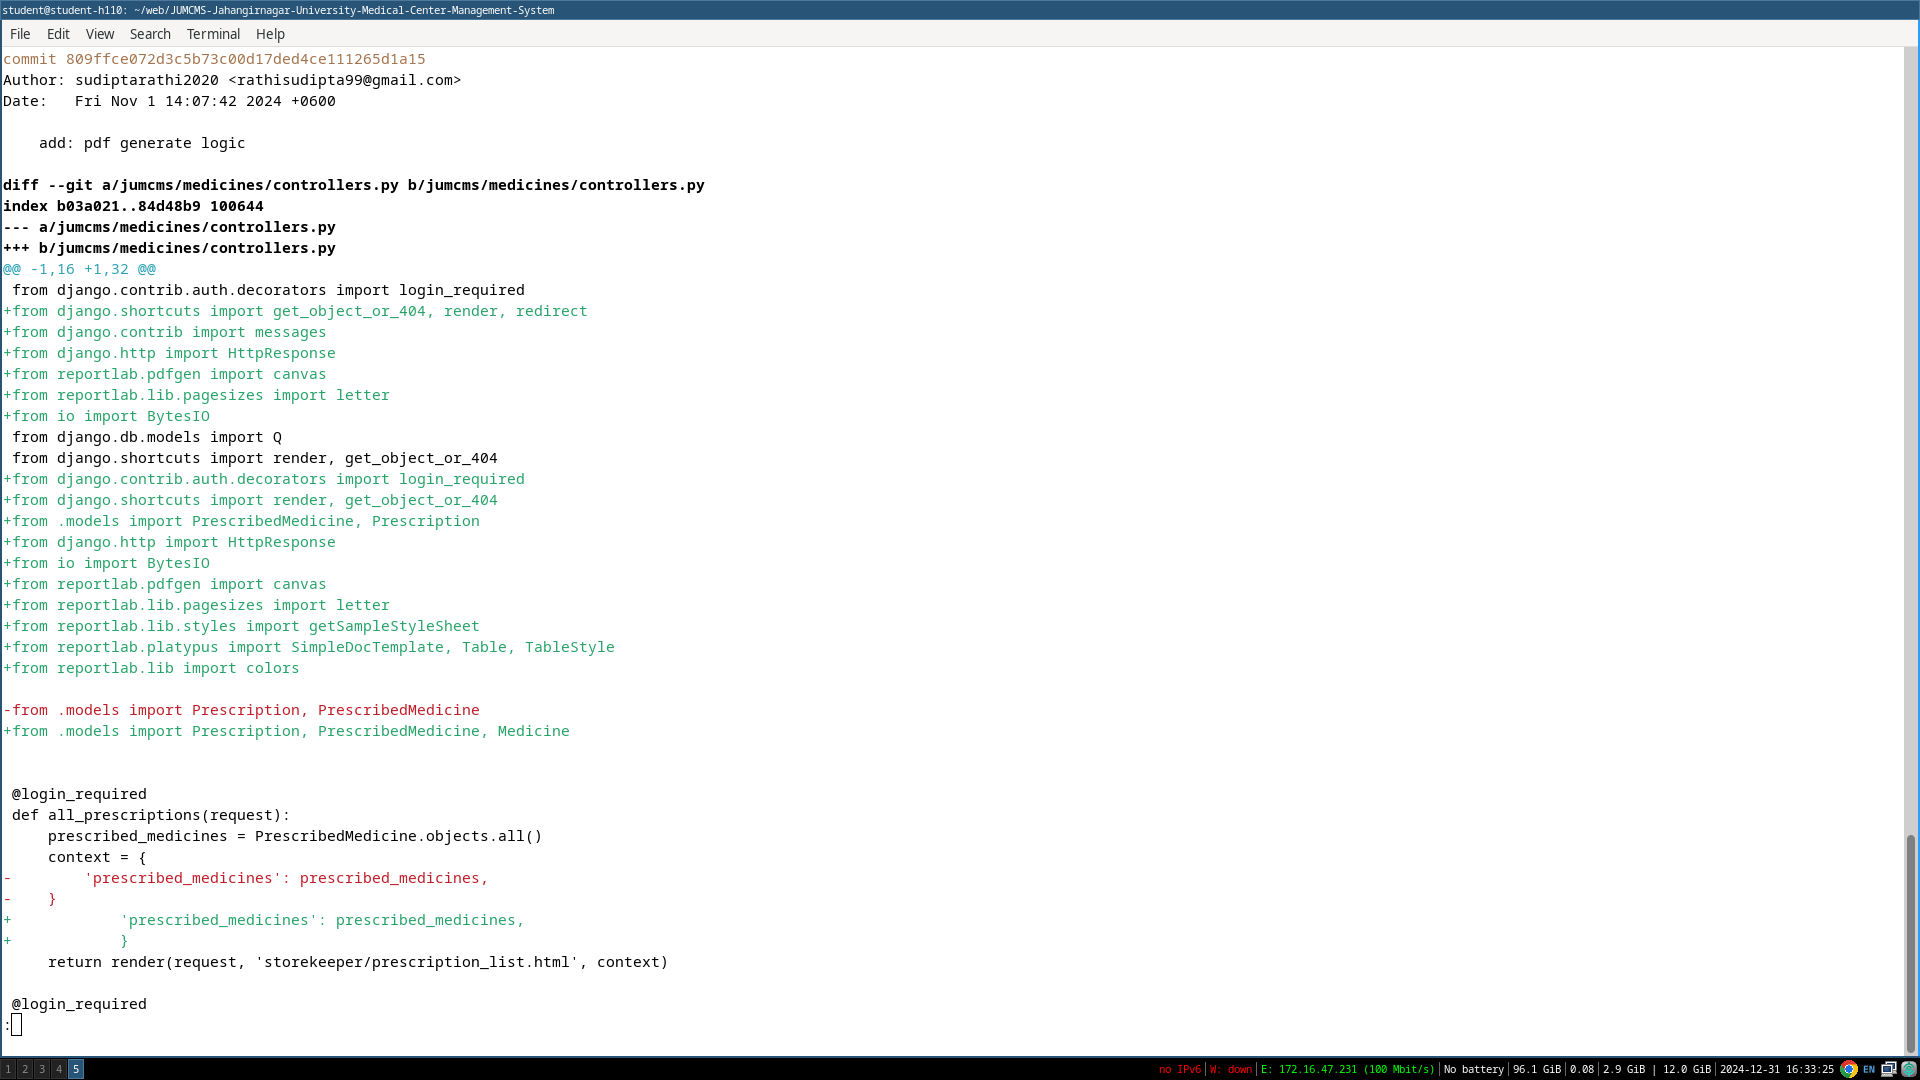
\includegraphics[width=1\textwidth]{images/scr2git3.png}
    \caption{Git log for pdf generate logic}
    \label{fig:gitlogscr23}
\end{figure}

\begin{figure}[H]
    \centering
    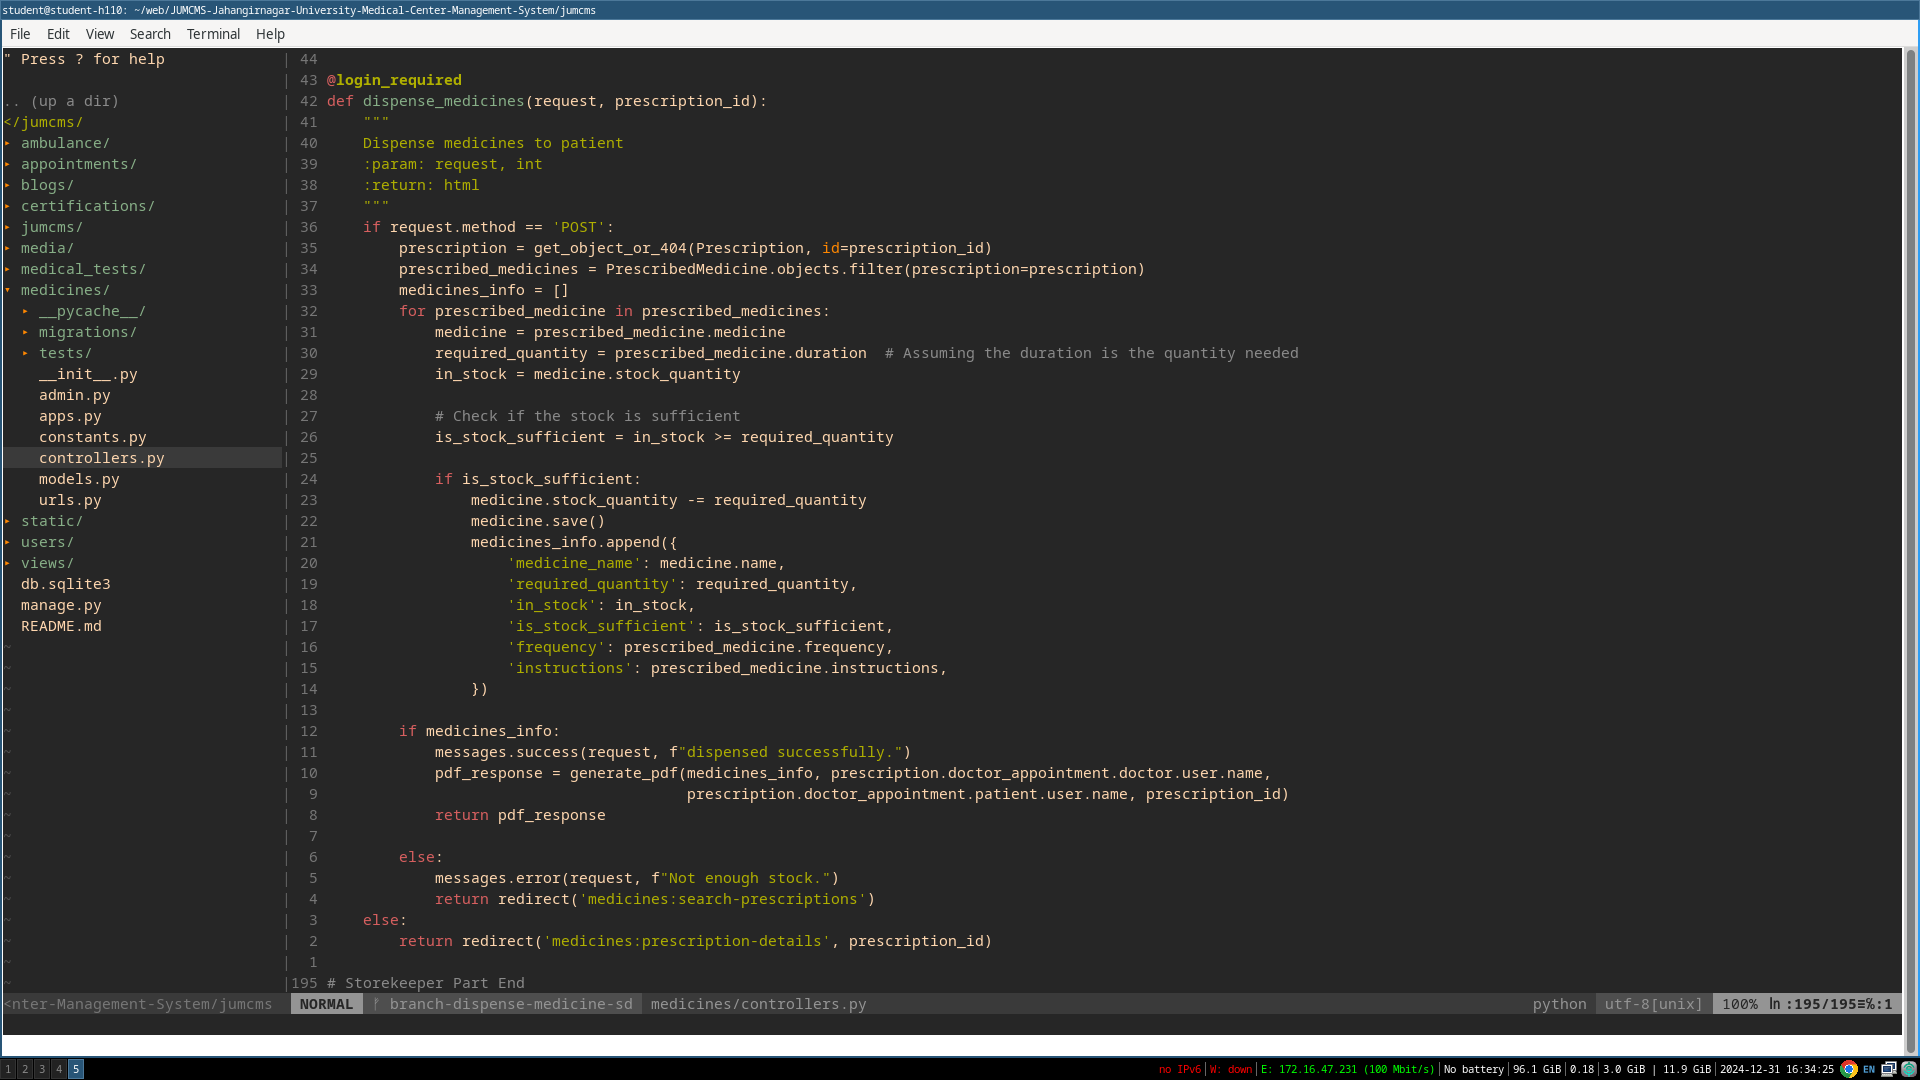
\includegraphics[width=1\textwidth]{images/scr2examplecode1.png}
    \caption{Example code for dispense medicine}
    \label{fig:scr2code1}
\end{figure}

\begin{figure}[H]
    \centering
    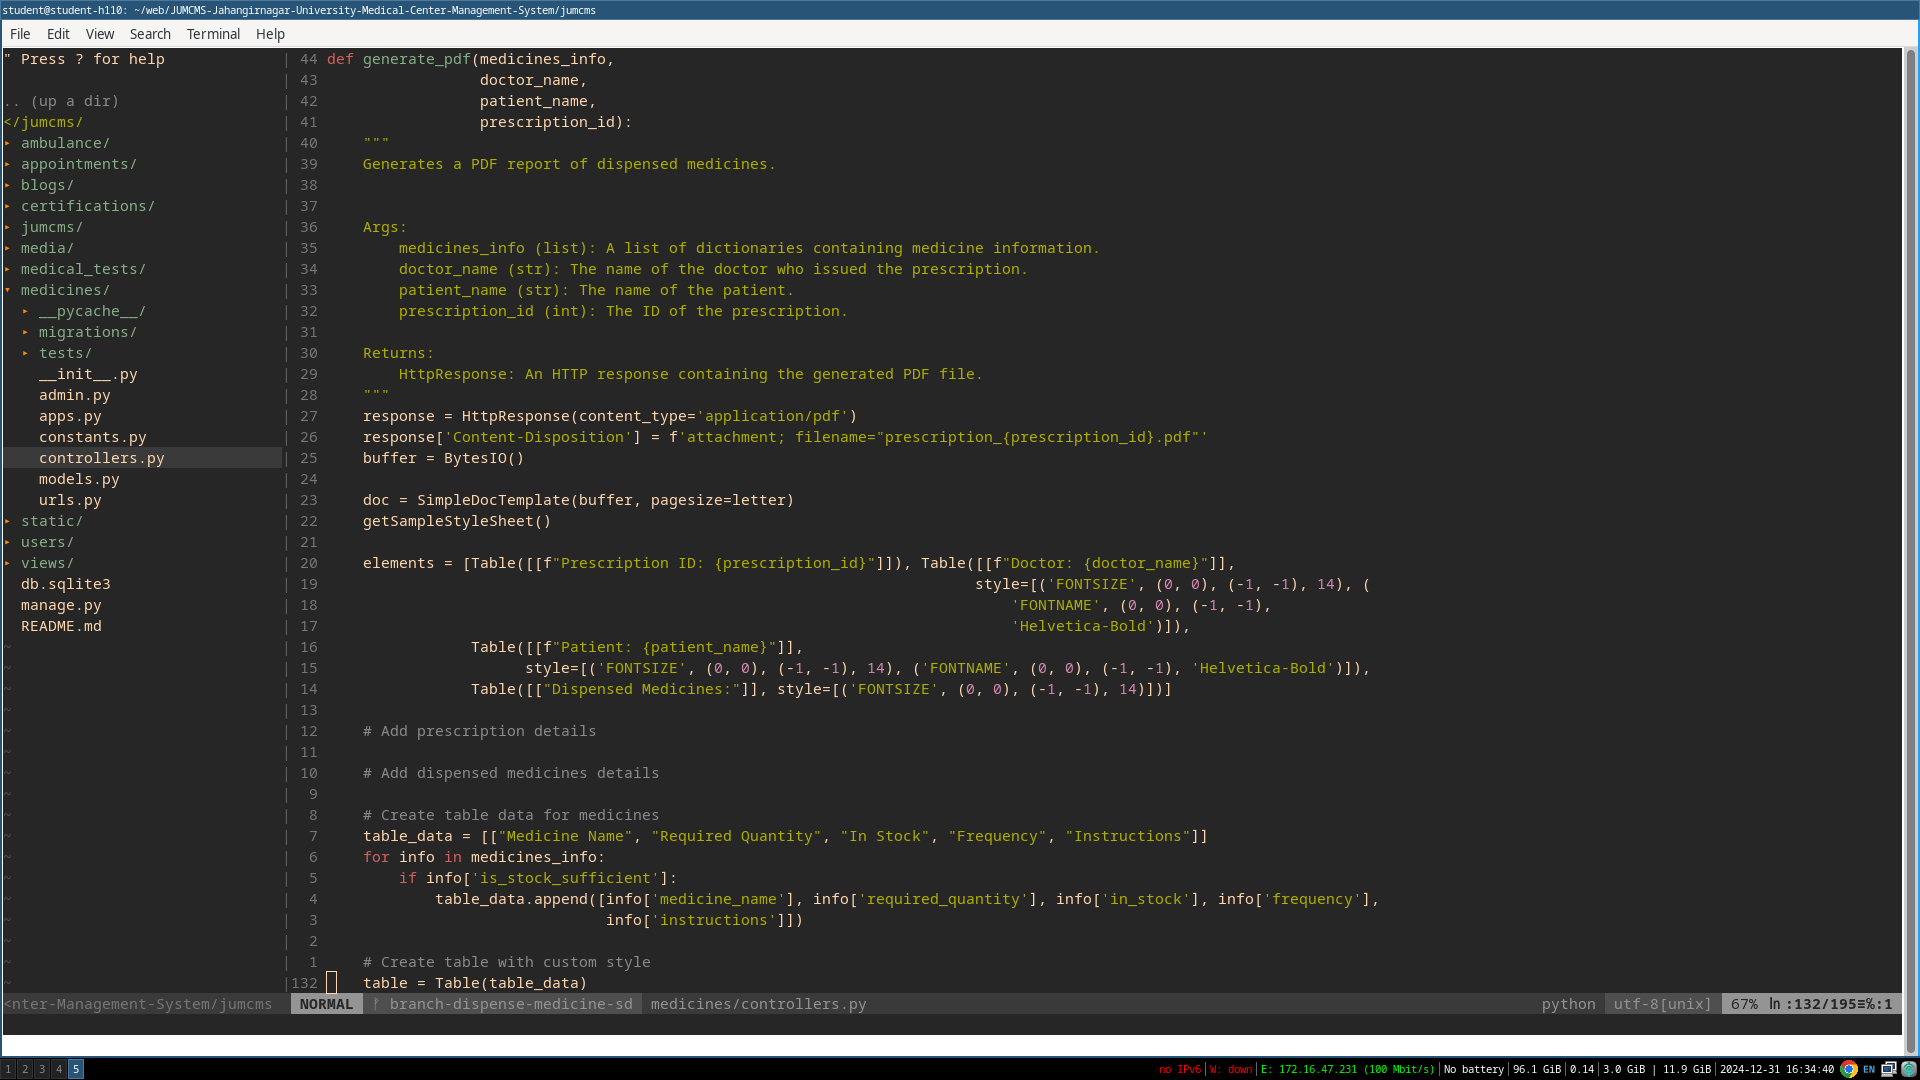
\includegraphics[width=1\textwidth]{images/scr2examplecode2.png}
    \caption{Example code for dispense medicine}
    \label{fig:scr2code2}
\end{figure}


\begin{figure}[H]
    \centering
    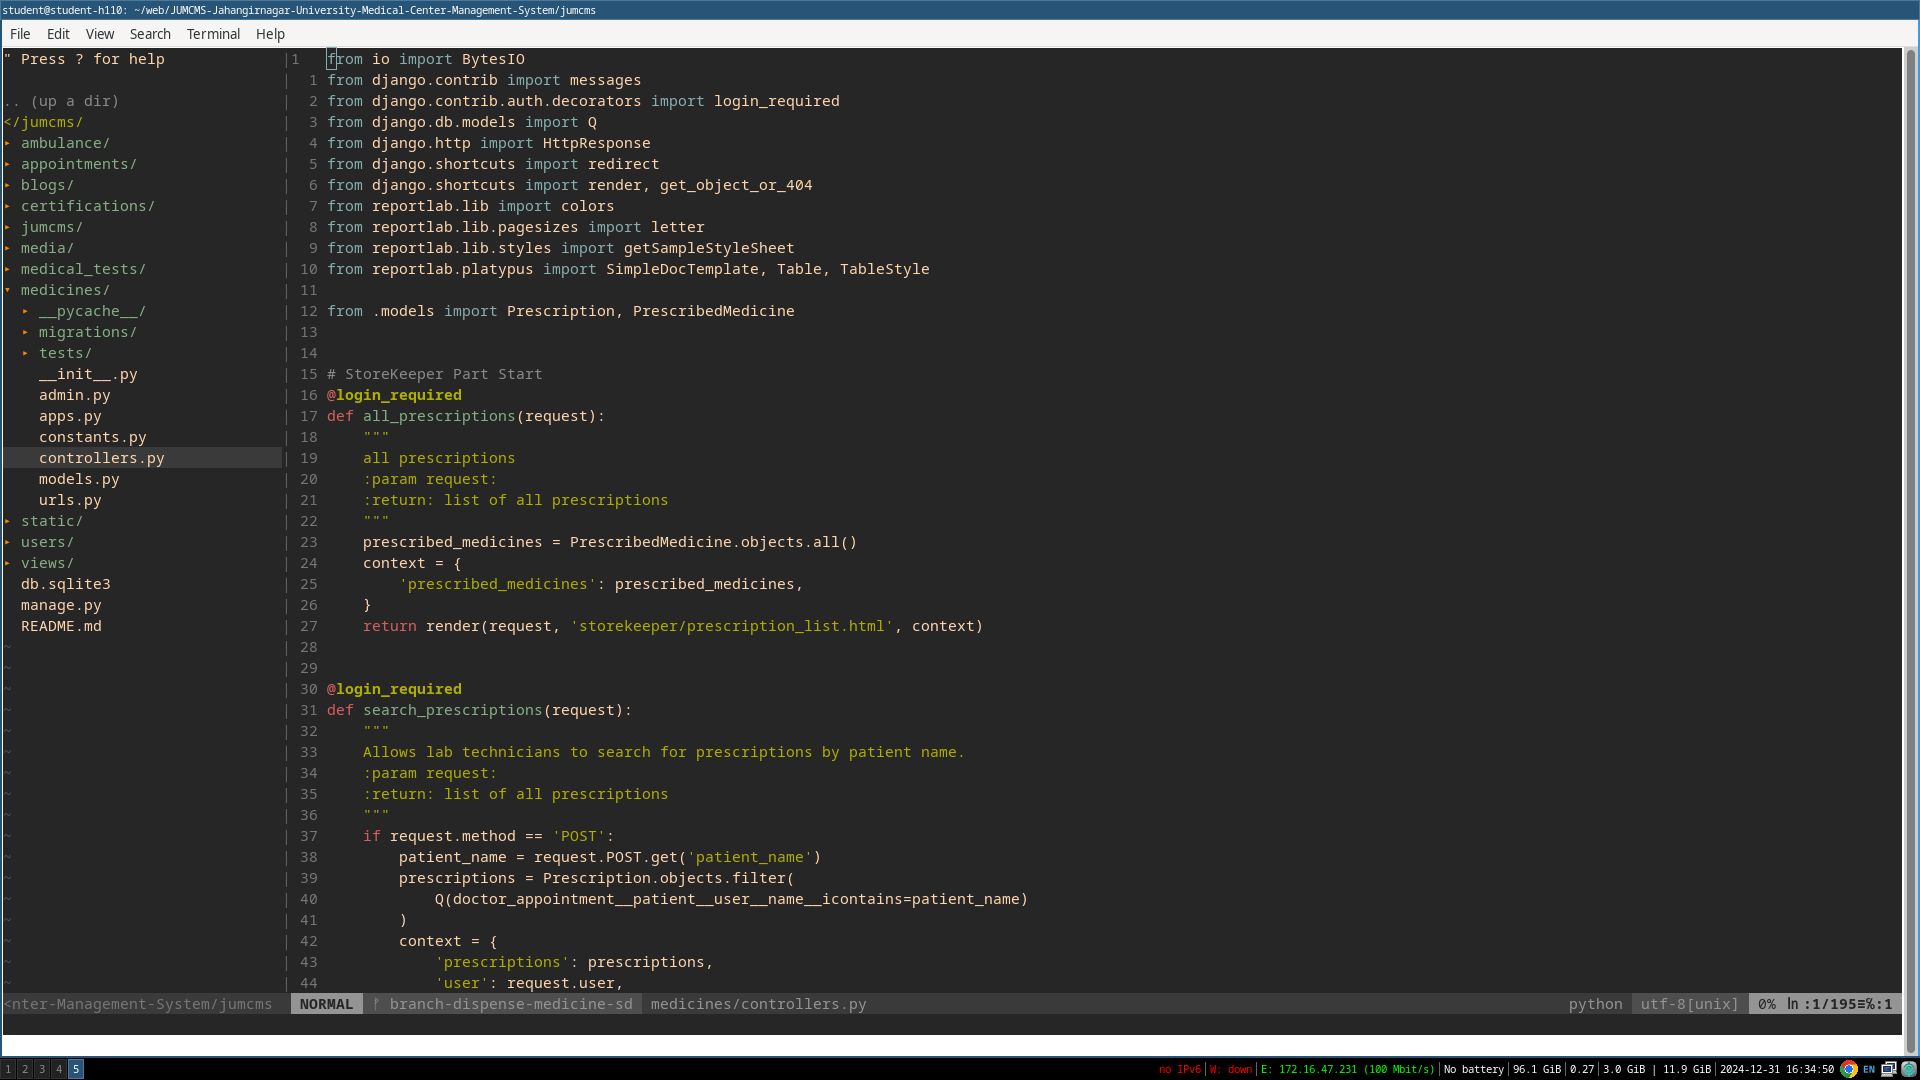
\includegraphics[width=1\textwidth]{images/scr2examplecode3.png}
    \caption{Example code for dispense medicine}
    \label{fig:scr2code3}
\end{figure}


\subsection{Scrum Meeting Update 3}
\begin{itemize}
    \item Added test case for dispense medicine feature
    \item Faced Some challenges in URL Routing
    \item Discussed with Subarna Saha to solve URL routing
\end{itemize}

\begin{figure}[H]
    \centering
    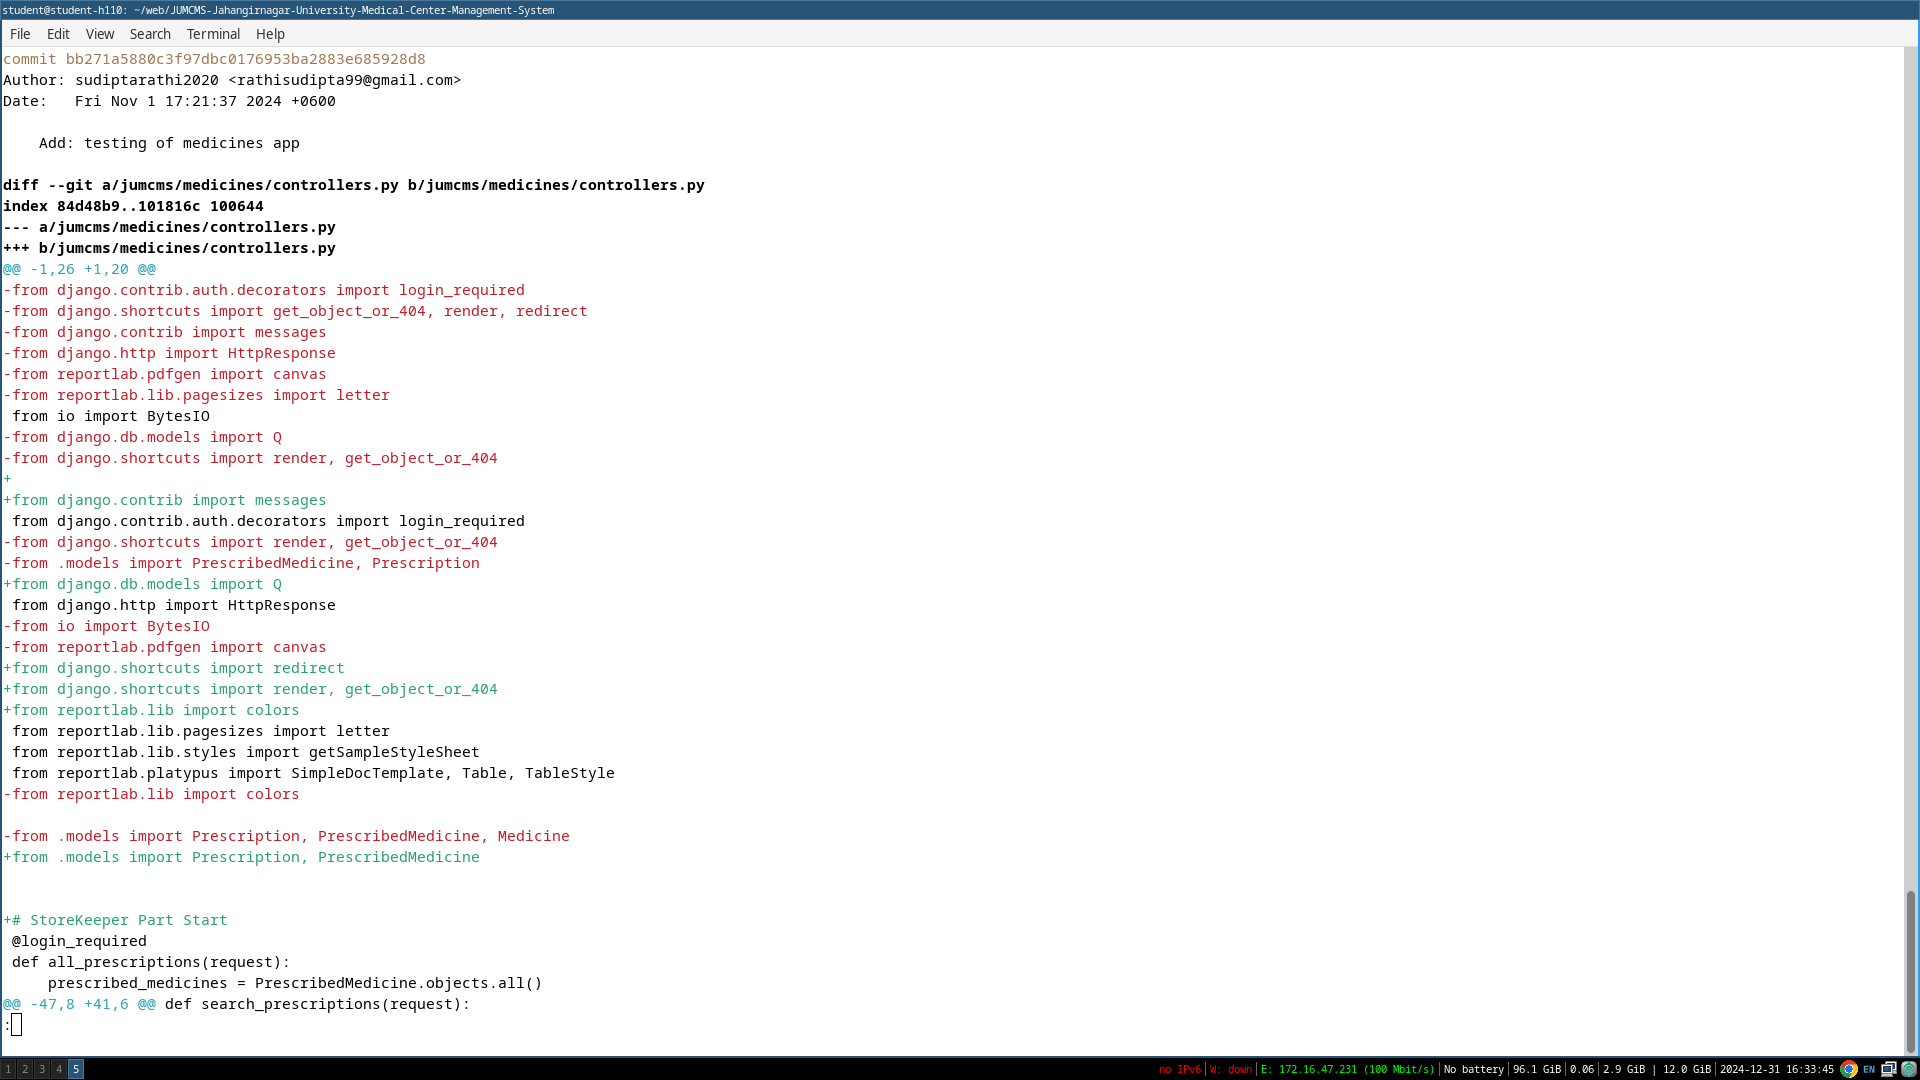
\includegraphics[width=1\textwidth]{images/scr2git4.png}
    \caption{Git log for Test case}
    \label{fig:gitlogscr24}
\end{figure}

\begin{figure}[H]
    \centering
    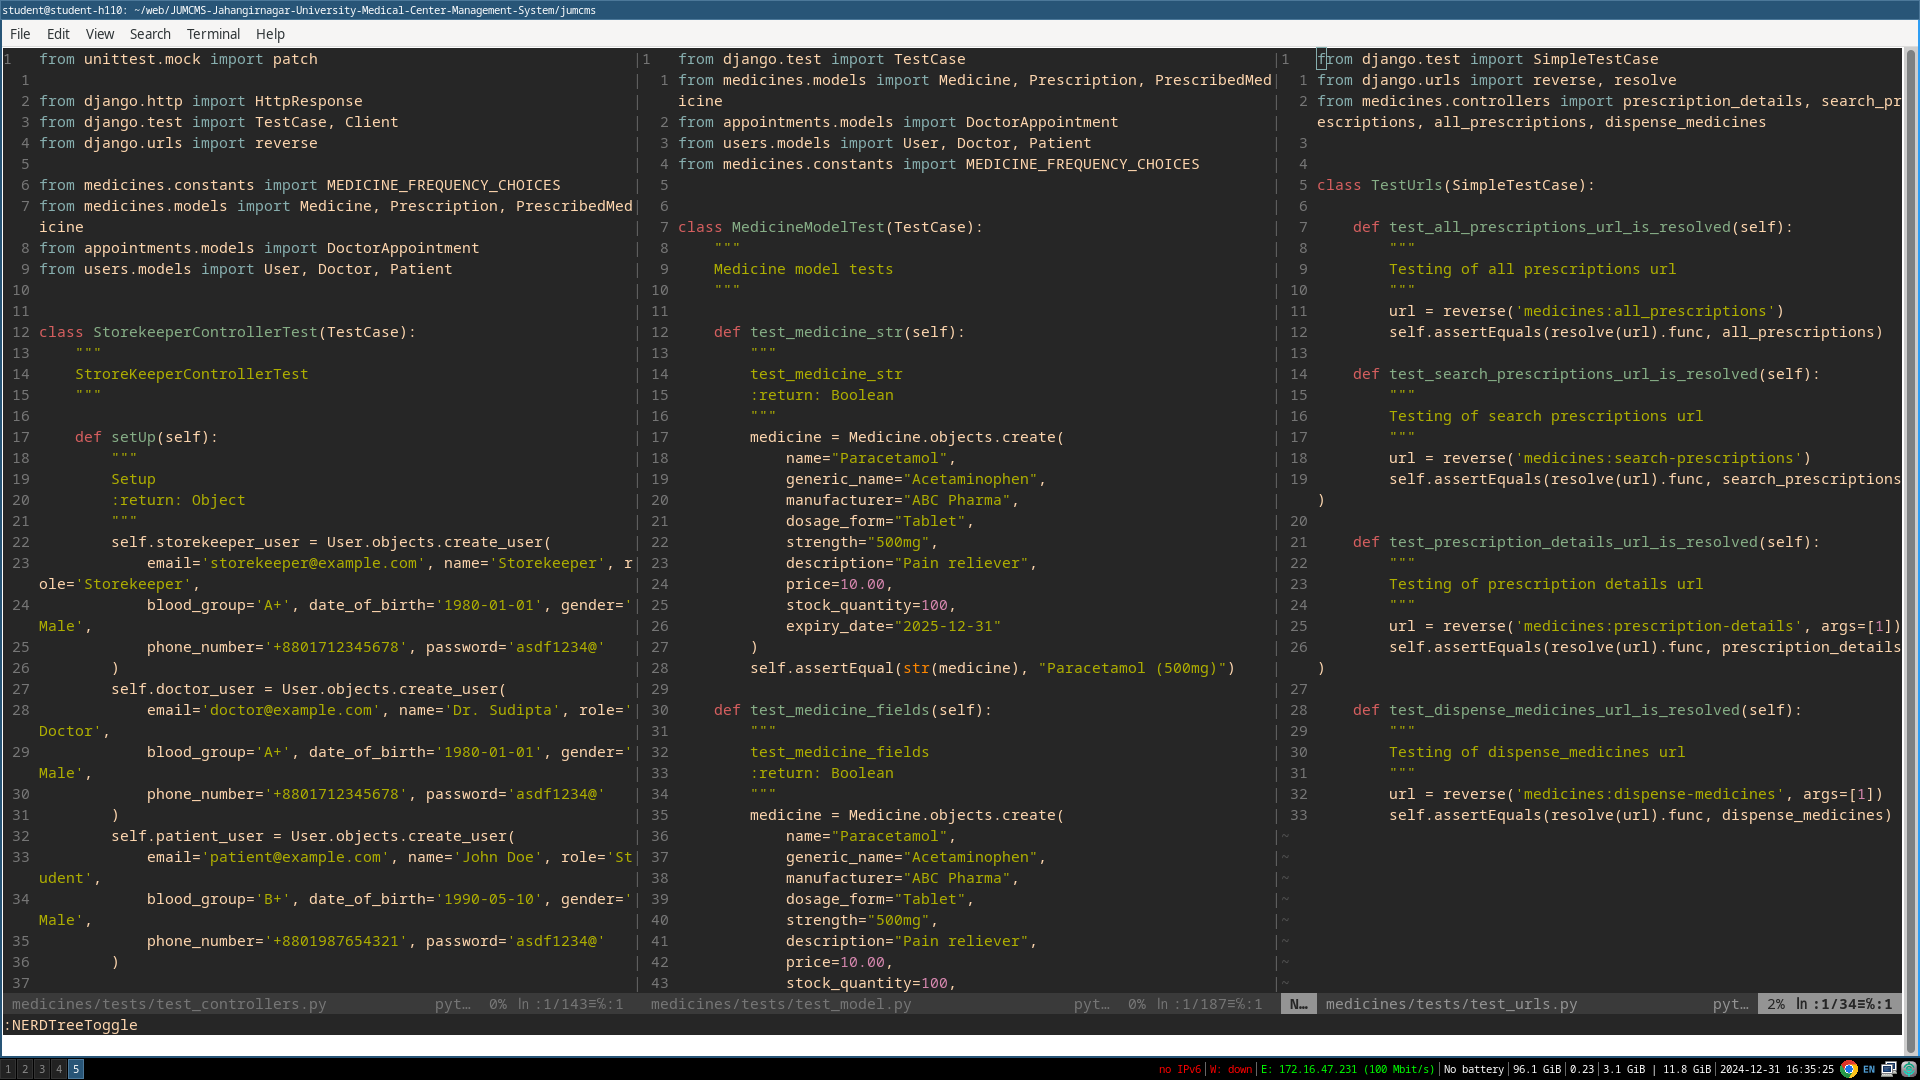
\includegraphics[width=1\textwidth]{images/src2test.png}
    \caption{Test Case Code for Dispense medicine}
    \label{fig:testcodefordispensemedicine}
\end{figure}

\begin{figure}[H]
    \centering
    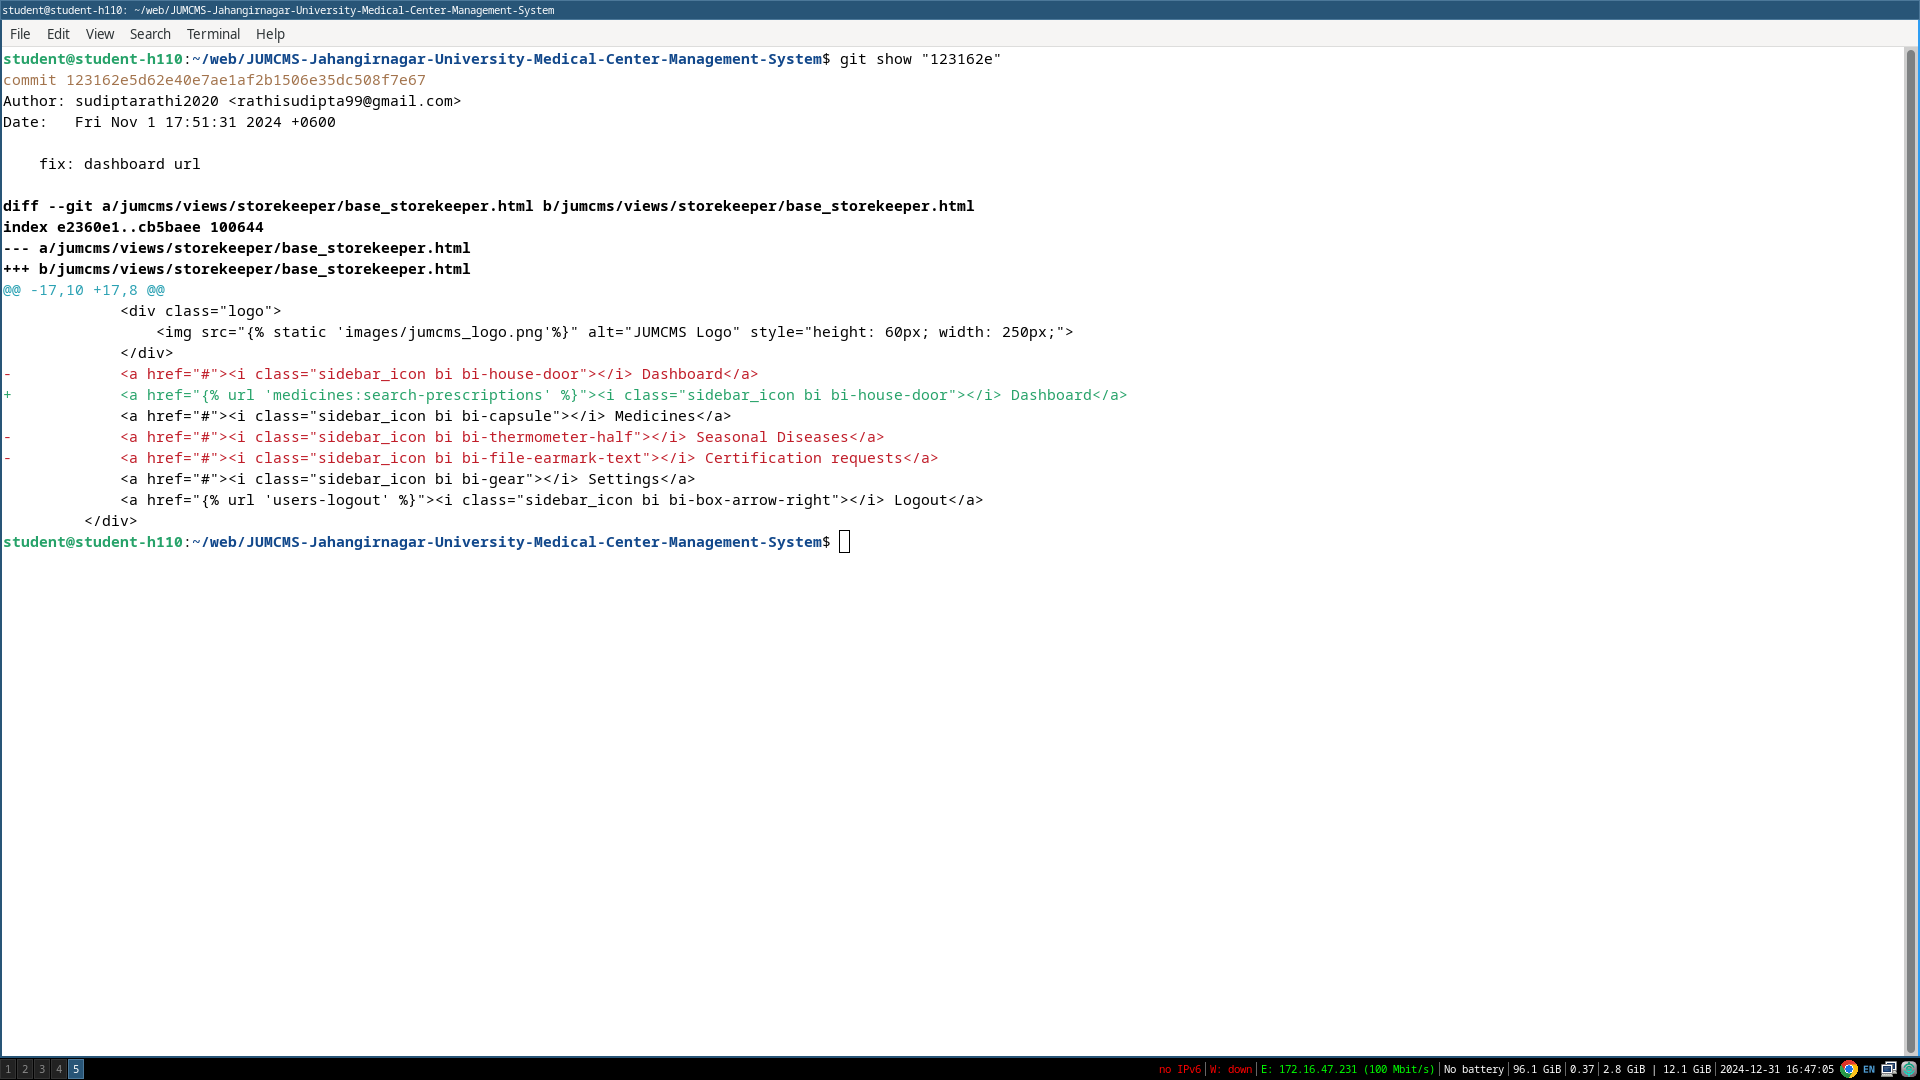
\includegraphics[width=1\textwidth]{images/scr3url.png}
    \caption{URL routig}
    \label{fig:urlrouting}
\end{figure}
\end{document}
